\newpage
\appendix
\onecolumn


\section{Convergence Proof of \methodname{}}
\label{app:convergence_proof}

\subsection{A Warm-Up Argument for a Single Offspring }

The overall goal of this section is to prove Theorem~\ref{theo:multipleOffspring}. As the main argument is quite complex, relying heavily on stochastic drift analysis, we begin with a warm-up, namely by presenting a simpler proof for the restricted case where $\lambda=1$.

Unlike the practical application of Algorithm~\ref{alg:1+lambda}, this section assumes that each fitness evaluation returns the exact, or 'true,' fitness value, ignoring any noise introduced by minibatching. Additionally, our results hold for any initialization.  To align with standard notation in the runtime analysis of evolutionary algorithms, we will count generations starting from zero (i.e., using 0-based indexing).

\begin{theorem}[Single offspring] \label{theo:singleOffspring}
    Let $n,k \in \mathbb{N}$ with $k \le n$ and consider the \opoea with level-switch mutation. Then any linear fitness function  $f: \{\mathbf{x}\;|\; \mathbf{x} \in \{0,1\}^n, \| \mathbf{x} \|_1=n-k \} \rightarrow \mathbb{R}$ is optimized in expected  
    \begin{displaymath}
        O(k\cdot (n-k)) \textnormal{ generations.}
    \end{displaymath}
    
\end{theorem}
\begin{proof}
Let $w \in \mathbb{R}^n$ be the weights associated with the linear function such that $f(x) = \sum_{i=1}^n x_i \cdot w_i$. To derive an upper bound, we can assume that no two weights are equal\footnote{Formally, this can be shown using stochastic domination, which involves coupling the potentials in both cases and proving that, given the same randomness, one is always at least as large as the other.}. Furthermore, assume without loss of generality that these weights are sorted increasingly, meaning $w_1 < w_2 < ... < w_n$, and that $k \le (n-k)$, as the other case follows from symmetry. Since $f$ is defined on the bit strings with exactly $k$ 0's its unique optimum is now given by $x_{\text{opt}}=0^{k} 1^{n-k}$. Denote by $x^{(t)}$ the search point at step $t$ and let 
\begin{displaymath}
T = \inf\{ t \geq 0 \mid x^{(t)} = x_{\text{opt}}\}
\end{displaymath}
be the number of generations required until the optimum is found. \\
Define $X^{(t)} = \sum_{j=1}^k x^{(t)}_j$ as the random variable that captures the number of $1$'s in the first $k$ bits of the search point at step $t$. We observe the following:
\begin{enumerate}
    \item $X^{(t)} = 0 \Leftrightarrow x^{(t)} = x_{\text{opt}}$;
    \item $X^{(t)}$ is non-increasing;
    \item $X^{(t)}-X^{(t+1)} \le 1$;
    \item $X^{(0)} = \sum_{j=1}^k x^{(0)}_j$.
\end{enumerate}
It follows that given the initial search point $x^{(0)}$ we can decompose $T$ into $s=\sum_{j=1}^k x^{(0)}_j$ stages $T_1, T_2, ..., T_s$, where $T_j = \inf(\{t \ge 0 \;|\; X^{(t)}=j-1\})- \inf(\{t \ge 0 \;|\; X^{(t)} = j\})$ captures the number of generations spent at stage $j$. By the linearity of expectation, we have
\begin{displaymath}
    \mathbb{E}[T \;| \;X^{(0)} = s] = \sum_{j=1}^{s} \mathbb{E}[T_j].
\end{displaymath}
It remains to bound the expected time spent at each stage. Each offspring is generated by copying the parent, selecting a $1$-bit uniformly at random, selecting a $0$-bit uniformly at random, and finally flipping both bits. At stage $j$ exactly $j$ of the $k$ $0$-bits are among the last $n-k$ positions and exactly $j$ of the $n-k$ $1$-bits are among the $k$ first positions. Hence, $j^2$ out of the total $k(n-k)$ ($1$-bit position, $0$-bit position)-pairs advance the optimization to the next stage, yielding
\begin{displaymath}
        \mathbb{P}[X^{(t+1)} = j-1 \; | \; X^{(t)}=j] = \frac{j^2}{k(n-k)}.
\end{displaymath}
Therefore, $T_j \sim \text{Geometric}(\frac{j^2}{k(n-k)})$ and
\begin{displaymath}
    \mathbb{E}[T_j] = \frac{k(n-k)}{j^2}.
\end{displaymath}

To obtain an upper bound, we can make a worst-case assumption by setting $X(x^{(0)}) = k$. We conclude
  \begin{displaymath}
      \mathbb{E}[T] \le \mathbb{E}[T | X^{(0)} = k] = \sum_{j=1}^k \mathbb{E}[T_j] = k(n-k) \sum_{j=1}^k \frac{1}{j^2} \in O(k(n-k)).
  \end{displaymath} 
\end{proof}

\paragraph{Discussion.} Observe that, under the assumption that the probability of initializing at the optimum is sufficiently small, the proof is tight up to a constant factor of 2.


It is important to note that the above proof relies on the key assumption that whenever one of the $j^2$ ``good'' pairs is selected during mutation, the resulting offspring is the fittest among all candidates. This condition holds naturally when there is only a single offspring, as the offspring produced by flipping one of the $j^2$ pairs will have higher fitness than the parent. However, in the case of multiple offspring, this approach breaks down, as an offspring produced by flipping one of the $j^2$ ``good'' pairs might still have lower fitness than another offspring that was not generated by flipping one of these $j^2$ ``good'' pairs.

\subsection{The Main Argument}

Drift analysis, originally developed to study all kinds Markov chains, has become the most widely used technique for analyzing the runtime of evolutionary algorithms in recent years. It works by first defining a potential function $X^{(t)}$ that measures the progress over each step $t$ of the optimization. By estimating how this potential changes at each step in expectation, i.e., computing the \emph{drift} in $X^{(t)}$, one can then make probabilistic statements about the  number of steps required until the potential reaches a certain threshold, also called the \emph{hitting time}. To this end, a variety of drift theorems have been established, two of which will be employed in our proof. For a more thorough introduction to drift analysis, we refer to \citet{drift_analysis_lengler}.


First of all, we will utilize the the Multiplicative Drift Theorem, more specifically a tail bound introduced by Doerr and Goldberg, which is applicable when the potential decreases by a constant fraction in each step.
\vspace{3mm}
\begin{theorem}[Multiplicative Drift, Tail Bound \citep{doerr_tail_bounds}] \label{the:MDT,Tail}
Let $(X^{(t)})_{t\ge0}$ be a sequence of non-negative random variables over a finite state space $S \subset \mathbb{R}_0^+$. Assume that $X^{(0)} \le b$ and let $T$ be the random variable that denotes the first point in time $t \in \mathbb{N}$ for which $X^{(t)} \le a$, for some $a \le b$. Suppose that there exists $\delta > 0$ such that for all $t < T$, 
\begin{displaymath}
    \mathbb{E}[X^{(t)}-X^{(t+1)} \; | \; X^{(t)}] \ge \delta X^{(t)}
\end{displaymath}
Then,
\begin{displaymath}
    \mathbb{P}[T > \frac{t+\log(b/a)}{\delta}]\le e^{-t}.
\end{displaymath}
\end{theorem}
\vspace{3mm}
Additionally, we will employ Johannsen's Variable Drift Theorem. This theorem provides more flexibility compared to the Multiplicative Drift Theorem, as it can be applied when the drift is bounded by any \emph{increasing} function of the potential. This often occurs naturally, as optimization typically becomes more difficult approaching the optimum.
\vspace{3mm}
\begin{theorem}[Variable Drift Theorem \citep{johannsen_phd_thesis}] \label{the:VDT}
Let $(X^{(t)})_{t\ge0}$ be a sequence of non-negative random variables over a finite state space $S \subset \mathbb{R}_0^+$. Let $s_{\text{min}} := \min(S \setminus \{0\})$, let $T := \inf\{t\ge0 \; |\; X^{(t)} = 0\}$, and for $s \in S$ let $\Delta^{(t)}(s) := \mathbb{E}[X^{(t)} - X^{(t+1)} \; |\; X^{(t)} =s]$. If there is an increasing function $h: \mathbb{R}^+ \rightarrow \mathbb{R}^+$ such that for all $s \in S \setminus \{0\}$ and all $t \ge 0$,
\begin{displaymath}
    \Delta^{(t)}(s) \ge h(s),
\end{displaymath}
then
\begin{displaymath}
    \mathbb{E}[T] \le \frac{s_{\text{min}}}{h(s_\text{min})} + \mathbb{E} \left[ \int_{s_\text{min}}^{X^{(0)}} \frac{1}{h(\sigma)}d\sigma \right],
\end{displaymath}
where the expectation on the latter term is over the random choice of $X^{(0)}$.
\end{theorem}
\vspace{3mm}

We will first prove an auxiliary lemma, which will play a central role in bounding the drift. For this purpose, we define an \emph{inversion} in a bit string $x\in \{0,1\}^n$ as a pair of indices $(i,j)$ such that $i<j$ and $x_i > x_j$. The distance between these indices, $j-i$, will be referred to as the \emph{spread} of this inversion.
\vspace{3mm}
\begin{lemma}
\label{lem:avgSpread}
    Let $x \in \{0,1\}^n$ be an arbitrary bit string with $k$ $0$-bits and denote by $s$ the number of inversions in $x$. Then, the average spread of these inversions is at least $\sqrt{s}/16$.
\end{lemma}
\begin{proof}
    Consider the bit string $1^{n-k}$ containing all $1$-bits of $x$. We can now generate an arbitrary bit string $x \in \{0,1\}^n$ with $k$ $0$-bits and $s$ inversions by adding $k$ $0$-bits in such a way that $s$ inversions are generated. Observe that adding a $0$-bit after the $j$'th $1$-bit results in exactly $j$ additional inversions, regardless of the other $0$-bits. This means that the order in which the $0$-bits are added does not affect the outcome. We proceed by a case distinction depending on how the inversions are generated.
    
    \vspace{2mm}
    \textbf{Case 1:} at least $s/2$ inversions are generated by adding $0$-bits after the $ \sqrt{s} $'th $1$-bit. 
    
    For each $0$-bit that is added after the $ \sqrt{s} $'th $1$-bit, at least half of the resulting inversions have spread at least $\sqrt{s}/2$. Consequently, this implies that there are at least $s/4$ inversions having spread at least $\sqrt{s}/2$ in total. 

    \vspace{2mm}
    \textbf{Case 2:} fewer than $s/2$ inversions are generated by adding $0$-bits after the $ \sqrt{s} $'th $1$-bit. 
    
    It follow that more than $s/2$ inversions are generated by adding $0$-bits not after the $\min(n-k,  \sqrt{s} )$'th $1$-bit. Observe that each $1$-bit can participate in at most $j$ inversions with spread at most $j$. More specifically, each $1$-bit can be part of at most $\sqrt{s}/4$ inversions with spread at most $\sqrt{s}/4$. Because all of the $s/2$ inversions that are added contain one of the first $\min(n-k,\sqrt{s})$ $1$-bits, at most $s/4$ of these inversions can have spread at most $\sqrt{s}/4$. Therefore, we conclude that the average spread of all inversions must be at least $\sqrt{s}/16$. 
\end{proof}
\vspace{3mm}
We continue to prove the final result. 

\vspace{3mm}
\paragraph{Proof of Theorem~\ref{theo:multipleOffspring}}

\begin{proof}
    As in the proof of Theorem~\ref{theo:singleOffspring} let $ w \in \mathbb{R}^n $ represent the weights associated with a linear function of the form $ f(x) = \sum_{i=1}^n x_i \cdot w_i $. To establish an upper bound, we can again assume that no two weights are equal. Additionally, without loss of generality, assume that the weights are ordered in increasing value, i.e., $ w_1 < w_2 < \dots < w_n $, and that $ k \leq n - k $, as the other case follows by symmetry. Let $ x^{(t)} $ denote the search point at step $ t $, and define 
    \begin{displaymath}
    T = \inf\{ t \geq 0 \mid x^{(t)} = 0^{k}1^{n-k} \}
    \end{displaymath}
    as the number of generations required to reach the optimal solution. \\
    Consider the potential function 
    \begin{displaymath}
    X^{(t)} = \sum_{i=1}^n (1-x^{(t)}_i) \cdot i - \frac{k \cdot (k+1)}{2},
    \end{displaymath} which captures the number of inversions at step $t$. Since $x_{\text{opt}} = 0^k 1^{n-k}$ is the only bit string with $k$ $0$-bits without inversions, we have $X^{(t)} = 0$ if and only if $x^{(t)}=x_{\text{opt}}$. At the same time, no bit string with $k$ $0$-bits has more than $k(n-k)$ inversions, hence, $X^{(t)} \le k(n-k)$ at all times. 
    During mutation, each of the $\lambda$ offspring is generated independently by copying the parent $x^{(t)}$, choosing uniformly at random one of the $1$-bits, choosing uniformly at random one of the $0$-bits and finally flipping both bits. This flipping can also be viewed as switching both bits, so that bits ``move'' across the search point in consecutive generations. We will use this abstraction in a later step of the proof. 
    
    As we assume the weights to be ordered increasingly, an offspring is fitter than its parent if and only if the chosen $1$-bit was to the left of the chosen $0$-bit, meaning, the chosen pair during mutation was an inversion. Since there are $k(n-k)$ possible pairs in total, we have for each offspring $y_1, ..., y_{\lambda}$
    \begin{displaymath}
        \mathbb{P}[f(y_j) > f(x^{(t)}) \;|\; X^{(t)}= s] = \frac{s}{k(n-k)}.
    \end{displaymath}
    At the same time, switching two bits corresponding to an inversion decreases the number of inversions by the difference in their positions, which we call the \emph{spread} of an inversion. This implies that any offspring fitter than its parent must have fewer inversions than its parent and therefore, $X^{(t+1)} \le X^{(t)}$ for all $t$. Note that we cannot make the same statement about the entire group of offspring, meaning, the fittest offspring is not guaranteed to have the fewest inversions. Since $X^{(t)}$ is non-increasing we can decompose $T$ into the number of steps required until for the first time the current search point $x^{(t)}$ has at most  $ k(n-k)/\lambda$ inversions and the number of steps required from there until the optimum is found. By linearity of expectation
    \begin{displaymath}
        \mathbb{E}[T] = \mathbb{E}[T_1] + \mathbb{E}[T_2],
    \end{displaymath}
    where
    \begin{displaymath}
    T_1 = \inf\{ t \ge 0 \mid X^{(t)} \le  \frac{k(n-k)}{\lambda}\}
    \end{displaymath}
    and
    \begin{displaymath}
        T_2= \inf\{ t \ge 0 \mid X^{(t)} = 0 \} - \inf\{ t \ge 0 \mid X^{(t)} \le \frac{k(n-k)}{\lambda} \}.
    \end{displaymath}

    In the remainder of this proof we will demonstrate that each of these two phases requires only an expected $O(k(n-k)/\lambda)$ generations.
    
    \vspace{4mm}
    We begin by bounding the expected number of steps until the search point has at most $k(n-k)/\lambda$ inversions. As computed previously, a single offspring is fitter than its parent with probability $\frac{s}{k(n-k)}$. Since any fitter offspring has fewer inversion than its parent, the potential decreases in a given step, if and only if, at least one of the offspring is fitter. By using that each offspring is generated independently and that $s \ge \frac{k(n-k)}{\lambda}$ for this phase we get that 
    \begin{displaymath}
        \mathbb{P}[X^{(t+1)} < X^{(t)} \; | \;X^{(t)}=s] = 1-(1-\frac{s}{k(n-k)})^\lambda \ge 1-e^{\frac{-\lambda s}{k(n-k)}} \ge 1 - e^{-1}.
    \end{displaymath}
    This means, in phase $1$ we have a constant probability of decreasing the potential every step. However, the resulting constant drift only provides an upper bound of $O(k(n-k))$ via the Additive Drift Theorem \citep{he_ADT}. Improving this constant drift bound is challenging because we must establish a lower bound on the expected reduction in the number of inversions, given the existence of a fitter offspring. The number of inversions in an offspring is not independent of its fitness, and there is no guarantee that a fitter offspring will have fewer inversions than a less fit one. This issue is mitigated when there is only a single fitter offspring (as demonstrated in the proof of phase 2), but it becomes problematic when multiple offspring are fitter than the parent with high probability. For example, consider the bit string $1^10^{10}1^{100}0^1$ with corresponding weights $w_1=1,w_2=1002,w_3=1003, ..., w_{112}=1112$. If $\lambda$ is reasonably large it becomes very likely that at least one of the children will have the first $1$-bit chosen in mutation. This offspring is guaranteed to be the fittest one, but at the same time (assuming the chosen $0$-bit is not the last one) it decreases the number of inversions very little compared to sampling one of the inversions for mutation uniformly at random. We will resolve this difficulty by a separate drift argument.

 
    Let $B_C$ be the event that, within the next 
    \begin{displaymath}
    \frac{2C}{1-e^{-1}} \frac{k(n-k)}{\lambda}
    \end{displaymath}
    steps, the number of inversions in $x^{(t)}$ falls below the threshold of 
    \begin{displaymath}
    \frac{k(n-k)}{\lambda}.
    \end{displaymath}
    Here, $ C $ is chosen such that $ \lambda \leq \frac{C}{8} \frac{n}{\log(n)} $. If we can demonstrate that $ B_C $ occurs with a probability of at least some constant, then the proof of the first phase is established, as $ B_C $ is expected to occur after a constant number of repetitions.
    
    Henceforth, we will implicitly condition on $ s \geq k(n-k) /\lambda $, since otherwise, the conclusion follows immediately. By the Chernoff bound over round events, the probability that the potential decreases at most 
    \begin{displaymath}
    C \frac{k(n-k)}{\lambda}
    \end{displaymath}
    times within the next 
    \begin{displaymath}
    \frac{2C}{1-e^{-1}} \frac{k(n-k)}{\lambda} 
    \end{displaymath}
    rounds is sub-constant. We will condition on the event that the potential decreases at least 
    \begin{displaymath}
    C \frac{k(n-k)}{\lambda}
    \end{displaymath}
    times, and from now on, we will only consider such potential-reducing generations.

    If we regard mutation as swapping the $1$-bit with the $0$-bit, we can enumerate all $0$-bits from $1$ to $k$ and denote by $i_j$ the current position of the $j$'th $0$-bit, which will be referred to as $0_j$. Note that this enumeration stays fixed across generations, meaning that the relative order can change and $0_j$ is not necessarily the $j$'th $0$-bit in $x^{(t)}$. Now define 
    \begin{displaymath}
    Z^{(t)}_j = 1+\sum_{l=1}^{i_j} x^{t} 
    \end{displaymath}
    as the random variable that captures the number of $1$-bits before $0_j$ plus one, or in other words, one plus the number of inversions this specific $0$-bit is part of. Let $S_j$ denote the event that the fittest offspring was generated by a mutation that selected $0_j$ and this offspring is fitter than the parent. We continue to show that
    \begin{displaymath}
    \mathbb{E}[Z^{(t+1)}_j \;|\; Z_j^{(t)}=s, S_j] \ge \frac{s}{2}.
    \end{displaymath}
    We achieve this by systematically revealing the randomness in each generation. First, uncover which $0$-bit flip produced the fittest offspring\footnote{More precisely, we must uncover which $0$-bit flip resulted in the offspring selected during the selection process. This accounts for scenarios where multiple offspring have the same highest fitness, in which case one of the fittest candidates is typically chosen uniformly at random. As the occurrence of multiple equally fit offspring is a mere technicality, we have largely omitted further discussion of this case.}. Assume this bit is $0_j$. Next, reveal all offspring that were generated by flipping other $0$-bits than $0_j$. Let $m$ be the number of offspring that were not uncovered yet, i.e., the number of offspring where $0_j$ was switched. Now enumerate all $1$-bits to the left of $0_j$ in $x^{(t)}$ from right to left (here, relative order matters). Let $l$ be the smallest integer such that when switching the $l$'th $1$-bit to the left of $0_j$ with $0_j$ the resulting offspring of $x^{(t)}$ has higher fitness than all $\lambda-m$ previously uncovered offspring. Denote by $D_l$ the corresponding event. Such $l$ must exists, since we condition on the event that some offspring with bit $0_j$ flipped (switched) is the fittest among all offspring. Because the weights are sorted increasingly it must hold that switching the $l+1$'th $1$-bit with $0_j$ will also result in an offspring with higher fitness than the other $\lambda - m$ offspring, while switching the $l-1$'th $1$-bit with $0_j$ will result in an offspring with lower fitness than the other $\lambda-m$ offspring. Next, uncover all offspring where bit $0_j$ was switched with one the first up to $(l-1)$'th bit to the left of $0_j$. Let $m'$ denote the number of yet uncovered offspring. Now each of the remaining $m'$ offspring is generated by flipping $0_j$ with one of the $l$'th to $(s-1)$'th $1$-bits to the left of $0_j$. Observe that the fittest among them will be the one with the leftest $1$-bit chosen. Therefore, 
    \begin{displaymath}
    \mathbb{E}[Z^{(t+1)}_j \;|\; Z_j^{(t)}=s, S_j, D_l, \text{$m'$ offspring not uncovered}] = s - \mathbb{E}\left[\max_{i=1,...,m'} U_i\right],
    \end{displaymath}
    where $U_i \sim \text{Uniform}(l, s-1)$. Given that we are conditioning on $S_j$, we know that the fittest offspring was produced by flipping $0_j$, which implies $m' \ge 1$. As $l \ge 1$ it follows that
    \begin{displaymath}
     \mathbb{E}[Z^{(t+1)}_j \;|\; Z_j^{(t)}=s,\; S_j] \ge s/2.
    \end{displaymath}

     Denote by $\hat{T_j}$ the number of steps required until $Z_j$ reaches $1$, only counting steps where $Z_j$ is decreased. Using a tail bound for the Multiplicative Drift Theorem (Theorem~\ref{the:MDT,Tail}) we have that 
    \begin{displaymath}
        \mathbb{P}[\hat{T_j} > 2(\log(n)+\log(n-k))] \le \frac{1}{n}.
    \end{displaymath}
    As $k < (n-k)$ we conclude by a union bound that with probability at least $1/2$ each potential $Z_j$ will reach $1$ within at most $4 \log(n)$ steps. Therefore, with probability at least $1/2$, after $4k\log(n)$ generations where some offspring is fitter than the parent, there must be $0$ inversions in $x^{(t)}$. Note that in practice, there will not actually be $0$ inversions in $x_t$, as the condition $s \ge k(n-k)/\lambda$ is violated earlier, leading the optimization process to enter the second phase. Using the fact that $\lambda \le \frac{C}{8}  \frac{n}{\log(n)}$ and $n-k \ge n/2$ we obtain
    \begin{displaymath}
        4k\log(n) \le \frac{8k(n-k) \log(n)}{n} \le C\frac{k(n-k)}{\lambda}.
    \end{displaymath}
    Finally, as the probability of having less than $C k (n-k) / \lambda$ ``successful'' generations in the considered time period is sub-constant, we conclude via another union bound that there exists a constant $C'$ such that event $B_{C}$ occurs with probability at least $1/C'$. Consequently, we have 
    \begin{displaymath}
        \mathbb{E}[T_1] \le C \cdot C' \cdot \frac{k(n-k)}{\lambda} \in O\left(\frac{k(n-k)}{\lambda}\right).
    \end{displaymath}


    \vspace{4mm}
    \looseness=-1
    To compute $\mathbb{E}[T_2]$ we first bound the probability that exactly one of the generated offspring is fitter than the parent. Denote by 
    \begin{displaymath}
    A_i = \left\{ \left| \left\{ j \in \{1, \dots, \lambda\} \mid f(y_j) > f(x^{(t)}) \right\} \right| = i \right\}
    \end{displaymath}
    the event that exactly $i$ of the offspring are fitter than the parent $x^{(t)}$. As shown earlier, the probability that a given offspring is fitter than its parent is exactly $\frac{s}{k(n-k)}$, where $s$ represents the number of inversions in $x^{(t)}$. Given that each offspring is generated independently, we have for $s \le k(n-k)/\lambda$
    \begin{align*}
    \mathbb{P}[A_1 \mid X^{(t)} = s] &= \lambda \cdot \frac{s}{k(n-k)} \cdot \left(1 - \frac{s}{k(n-k)}\right)^{\lambda-1} \\
    &\geq \lambda \cdot \frac{s}{k(n-k)} \cdot \left(1 - \frac{s}{k(n-k)}\right)^{\frac{k(n-k)}{s}-1} \\
    &\geq \lambda \cdot \frac{s}{k(n-k)} \cdot \frac{1}{e}.
\end{align*}

    Lemma \ref{lem:avgSpread} indicates that when selecting an offspring uniformly at random from all those with higher fitness than the parent (i.e., those generated by flipping an inversion), the expected number of inversions in that offspring is at least $\sqrt{s}/16$ fewer than in the parent. We can now reveal the randomness in two steps. First, we only uncover how many of the generated offspring are fitter than the parent. Given that there is only a single fitter offspring, i.e., conditioned on $A_1$, we then uncover its number of inversions. Clearly, this single fitter offspring is now sampled uniformly at random from all offspring with higher fitness than $x^{(t)}$; thus, for $s \le k(n-k)/\lambda$
    \vspace{1mm}
    \begin{align*}
    \Delta^{(t)}(s) &= \mathbb{E}[X^{(t+1)} - X^{(t)} \mid X^{(t)} = s] \\
    &= \sum_{k=0}^{\lambda} \mathbb{E}[X^{(t+1)} - X^{(t)} \mid X^{(t)} = s, A_k] \cdot \mathbb{P}[A_k \mid X^{(t)} = s] \\ 
    &\geq \mathbb{E}[X^{(t+1)} - X^{(t)} \mid X^{(t)} = s, A_1] \cdot \mathbb{P}[A_1 \mid X^{(t)} = s] \\
    &\geq \frac{\sqrt{s}}{16} \cdot \lambda \cdot \frac{s}{k(n-k)} \cdot \frac{1}{e}.
    \end{align*}

    Finally, applying Johannsen's Variable Drift Theorem \citep{johannsen_phd_thesis} (Theorem \ref{the:VDT}) yields
    \begin{align*}
    \mathbb{E}[T_2] &\leq  16e \frac{k(n-k)}{\lambda} + \mathbb{E}\left[\int_1^{X^{(0)}} 16e \frac{k(n-k)}{\lambda \sigma^{3/2}} \, d\sigma \right] \\
    &\leq 16e \frac{k(n-k)}{\lambda} \left( 1 + \int_1^{\frac{k(n-k)}{\lambda}} \frac{1}{\sigma^{3/2}} \, d\sigma \right) \\
    &\in O\left(\frac{k(n-k)}{\lambda}\right).
\end{align*}

\end{proof}

\section{Evolutionary Search Parameter Ablations}
\label{app:evo_search_ablations}
\subsection{Mutation Rate (Depth Pruning)}
\label{app:evo_search_ablations_dropping}

The mutation rate plays a crucial role in balancing exploration and exploitation. A higher mutation rate allows for broader exploration of the search space; however, this space grows exponentially with the number of mutations. As a result, when trying to approach the optimum in terms of Hamming distance, the proportion of ``good'' offspring decreases significantly with an increasing mutation rate. Consequently, in a smooth fitness landscape, we expect significantly faster optimization with a lower mutation rate.

To provide some mathematical intuition, consider optimizing over the $200$-dimensional hypercube $\{0,1\}^{200}$, where the current search point is $x^{(t)}=0^{200}$ and the global optimum is $x_{\text{opt}} = 1^{20} 0^{180}$. For this illustration we use a mutation operator that randomly selects a subset of $k$ bits to flip. Flipping $k$ bits corresponds to selecting a bitstring from the $k$'th Hamming layer of $x^{(t)}=0^{200}$ uniformly at random, where the $k$'th Hamming layer consists of all bitstrings with a Hamming distance of $k$ from $x^{(t)}$. Similarly, the Hamming ball of radius $k$ includes all bitstrings with a Hamming distance at most $k$. Assume that any bitstring closer to the optimum in terms of Hamming distance has higher fitness than our current search point\footnote{While this assumption does not hold in practice, it serves as a useful intuition in a reasonably smooth fitness landscape.}. The probability of improving the fitness via a mutation of $k$ bits equals the fraction of points in the $k$'th Hamming layer of $x^{(t)}$ that are also in the Hamming ball of radius $19$ around $x_{\text{opt}}$. When the current search point is reasonably close to the optimum, this ratio is maximized for $k=1$. For the described setting, we can compute the probabilities of each event $A_k$, where $A_k$ represents the event that mutating $k$ bits of $x^{(t)}$ results in a decrease in the Hamming distance from $x_{\text{opt}}$. These probabilities are given by: 
\[
\begin{array}{ll}
\mathbb{P}[A_1] = \frac{\binom{20}{1}}{\binom{200}{1}} = 0.1 
& \mathbb{P}[A_2] = \frac{\binom{20}{2}}{\binom{200}{2}} \approx 0.0095 \\  [10pt]
\mathbb{P}[A_3] = \frac{\binom{20}{3}+\binom{20}{2}\cdot \binom{180}{1}}{\binom{200}{3}} \approx 0.0269 &
\mathbb{P}[A_4] = \frac{\binom{20}{4}+\binom{20}{3}\cdot \binom{180}{1}}{\binom{200}{4}} \approx 0.0032 \\ [10pt]
\mathbb{P}[A_5] = \frac{\binom{20}{5}+\binom{20}{4}\cdot \binom{180}{1}+\binom{20}{3} \cdot \binom{180}{2}}{\binom{200}{5}} \approx 0.0076 & 
\mathbb{P}[A_6]= \frac{\binom{20}{6}+\binom{20}{5}\cdot \binom{180}{1} + \binom{20}{4} \cdot \binom{180}{2}}{\binom{200}{6}} \approx 0.0010
\end{array}
\]
 Note that accounting for the potentially greater Hamming distance gained for higher mutation rates (i.e., calculating the drift in the Hamming distance) has only marginal effect. This is because for an odd number of mutations, most of the conditional probability mass is concentrated on the case where the Hamming distance is reduced by just one bit. Similarly, for an even number of mutations, most of the conditional probability mass is concentrated on cases where the reduction in the Hamming distance is only two bits. The advantage of a low mutation rate becomes even more pronounced as the search process nears the optimum. For instance, when the Hamming distance between $x^{(t)}$ and $x_{\text{opt}}$ is 5, mutating a single bit results in a 16-fold greater drift in Hamming distance compared to any other mutation rate. 

To study the empirical impact of the mutation rate on our search process, we tested various distributions from which the number of mutations is sampled. Table~\ref{tab:ablation_mutation} illustrates the effects of these distributions for selecting the optimal twelve blocks to drop for Mistral-7B-v0.3. The results confirm our intuition: higher mutation rates generally reduce performance. However, sampling from the minimum of two uniform distributions ensures a reasonably high probability of choosing a low number of mutations. These offspring, with fewer mutations, then drive the optimization process, yielding comparably lower performance drops. Conversely, when we eliminate this sampling and instead use a high, constant mutation rate, we lose the locality that is crucial for evolutionary algorithms, leading to a significant drop in performance.

\begin{table}[htb]
\footnotesize
\centering
\setlength\tabcolsep{3pt}
\caption{Effect of varying the distribution determining the number of mutations.}

\resizebox{0.5\textwidth}{!}{
\begin{tabular}{c|ccc}
  \toprule
   \bf{Number of Mutations} & \bf{Wiki2$\downarrow$} & \bf{C4$\downarrow$} & \bf{FW$\downarrow$} \\
  \midrule
 
 \multicolumn{1}{l|}{$\min(U_1, U_2), \quad U_1, U_2 \sim U(1, 3)$}& \bf{17.52} & 21.60 & 16.79 \\
  \multicolumn{1}{l|}{$\min(U_1, U_2), \quad U_1, U_2 \sim U(1, 7)$} & 21.49 & 22.41 & 17.65 \\
 \multicolumn{1}{l|}{$\min(U_1, U_2), \quad U_1, U_2 \sim U(1, 15)$}& 18.65 & 22.67 & 17.63 \\
   \multicolumn{1}{c|}{$1$} & 18.12 & \bf{21.12} & \bf{16.33} \\
   \multicolumn{1}{c|}{$3$} & 22.09 & 25.42 & 19.25 \\
  \multicolumn{1}{c|}{$7$}& 25.06 & 26.52 & 19.65   \\
     \multicolumn{1}{c|}{$15$} & 27.01  & 28.19  & 22.03 \\
  \bottomrule
\end{tabular}
\label{tab:ablation_mutation}
}
\end{table}


A low mutation rate carries the risk of getting trapped in local optima. However, as discussed in Section~\ref{sec:method}, we expect dynamic model compression to exhibit a smooth fitness landscape with few local optima. Moreover, fitness evaluations in our context are relatively expensive. Increasing the mutation rate would only be beneficial if the smaller search space had already been thoroughly explored. In our case, though, even a small neighborhood cannot be fully explored within a feasible time frame.

A widely used strategy for balancing the advantages and disadvantages of different mutation rates involves self-adjusting mutation rates, which have been shown to be effective both theoretically and in practice \citep{kern_one_fifth_update_rule, doerr_lengler_self_adjusting_mutation}. These methods decrease the mutation rate when progress is relatively ``easy'', and increase it when progress becomes difficult, offering a greater chance of escaping local optima.



\subsection{Multi-Step Selection (Unstructured Sparsity)}
\label{app:evo_search_ablations_sparsity}
We will use this subsection to ablate the impact of hyperparameters for the multi-step selection, namely, the number of tokens and survivors. As discussed earlier in Section~\ref{subsect:sparsity}, the default hyperparameters we chose for our unstructured sparsity search were quite conservative. The following experiments will be conducted based on the ``super-fast'' version, which uses two steps of selection. It first generates $16$ offspring, evaluates them on $512$ tokens, and compares only the fittest one with the parent on another $8192$ tokens. 

Table~\ref{tab:ablation_tokens} shows the impact of adapting the number of tokens in the first selection step. Note that reducing tokens is only reasonable up to a certain degree, as fitness evaluation has constant overhead independent of the number of tokens (e.g., for loading the levels). Table~\ref{tab:ablation_offspring} ablates the number of offspring in each generation. All perplexities were measured after $400$ generations. 

\begin{table}[htb]

\footnotesize
\centering
\setlength\tabcolsep{3pt}
\caption{Effect of varying the number of tokens in first preselection step.}
\resizebox{0.6\textwidth}{!}{
\begin{tabular}{ccc|ccc}
  \toprule
  \bf{Offspring} & \bf{Stage 1: Tokens} & \bf{Stage 2: Tokens} & \bf{Wiki2$\downarrow$} & \bf{C4$\downarrow$} & \bf{FW$\downarrow$}  \\
  \midrule
  16 & 1024 & 8192 & 16.22 & \textbf{17.93} & \textbf{12.26} \\
  16 & 512 & 8192 & \textbf{15.87} & 18.28 & 12.38 \\
  16 & 256 & 8192 & 17.25 & 18.51 & 12.52 \\
  16 & 128 & 8192 & 16.01 & 18.99 & 12.72 \\
  16 & 64 & 8192 & 15.89 & 19.35 & 12.98 \\
  
  \bottomrule
\end{tabular}
\label{tab:ablation_tokens}
}
\end{table}

\begin{table}[htb]
\footnotesize
\centering
\setlength\tabcolsep{3pt}
\caption{Effect of varying the number of offspring.}
\resizebox{0.6\textwidth}{!}{
\begin{tabular}{ccc|ccc}
  \toprule
  \bf{Offspring} & \bf{Stage 1: Tokens} & \bf{Stage 2: Tokens} & \bf{Wiki2$\downarrow$} & \bf{C4$\downarrow$} & \bf{FW$\downarrow$} \\
  \midrule
    64 &  512 &  8192 & 16.35 & 18.27 &  \textbf{12.36} \\
    32 &  512 &  8192 & 16.65 & \textbf{18.22} & 12.44 \\
    16 &  512 &  8192 & \textbf{15.87} & 18.27 & 12.38 \\
    8 &  512 &  8192 & 16.37 & 18.74 & 12.64 \\
    4 &  512 &  8192 & 17.87 & 18.97 & 12.72 \\
  \bottomrule
\end{tabular}
\label{tab:ablation_offspring}
}
\end{table}


In a similar vein to the discussion in Appendix~\ref{app:evo_search_ablations_dropping}, the number of offspring can also be dynamically adapted. Ideally, the number of offspring should increase to the point where the computational effort is compensated by the number of generations, as outlined in Theorem~\ref{theo:multipleOffspring}. Methods such as the Self-Adjusting $(1,\lambda)$-EA have recently gained significant theoretical interest and have been shown to automatically determine ``ideal'' offspring sizes on specific problems \citep{sudholt_self_adjusting, kaufmann_self_adjusting}.



\subsection{Fitness Environment (Quantization)}
\label{app:evo_search_ablations_quantization}

We explored an alternative fitness function by testing perplexity as opposed to KL-Divergence. One advantage of using perplexity is the reduced memory requirement, as it does not necessitate storing the logits, which can be particularly burdensome for large vocabularies. However, perplexity relies solely on the information from the ground truth token, while KL-Divergence takes into account the entire distribution. This distinction is significant only if the selection decisions vary between the two metrics. Generally, we expect KL-Divergence to perform at least as well as perplexity; however, in many instances, their performances are similar. This observation could indicate that KL-Divergence might be using more tokens than necessary to assess fitness effectively. Although in the context of quantization KL-Divergence yielded slightly better results (Table~\ref{tab:ablation_fitness}, Figure~\ref{fig:ablation_fitness_klVsPPl} left), both metrics showed comparable performance when applied to unstructured sparsity (Figure~\ref{fig:ablation_fitness_klVsPPl} right).

\begin{figure}[htb]
    \centering
    % Left figure
    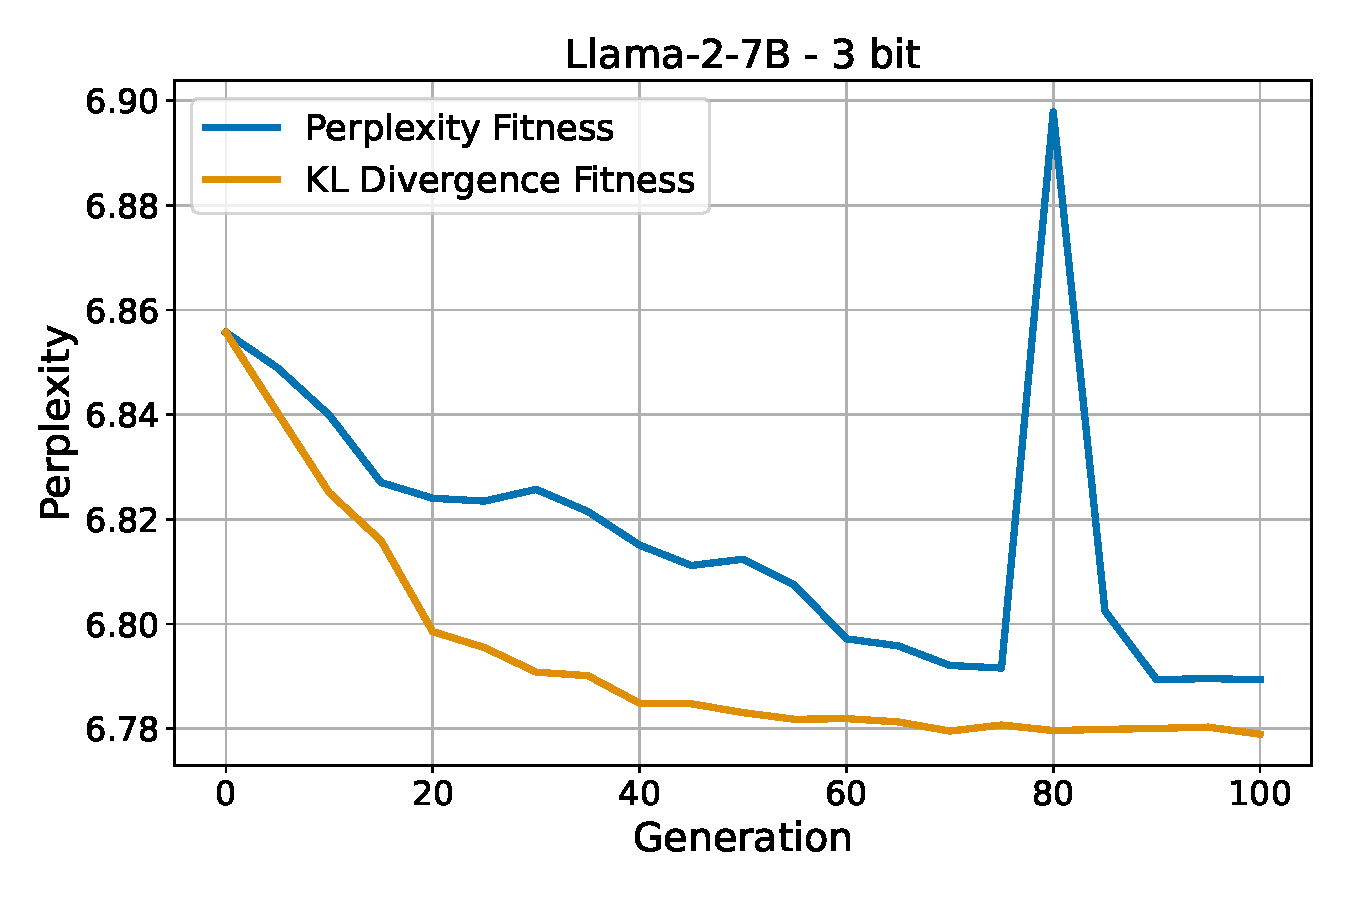
\includegraphics[width=0.48\linewidth]{graphics/Ablations/ablations_fitness_quant.pdf}
    \hfill
    % Right figure
    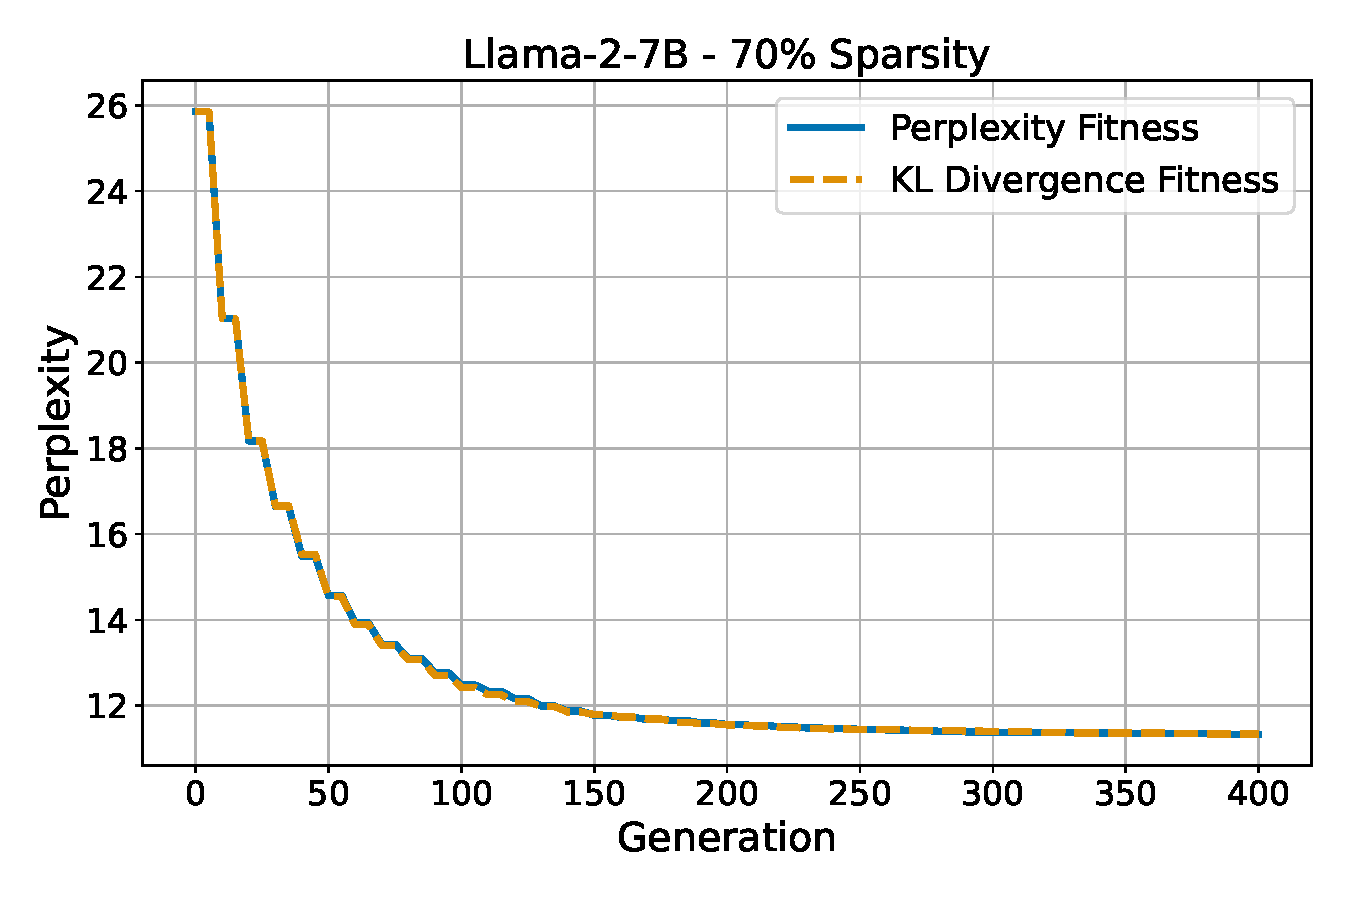
\includegraphics[width=0.48\linewidth]{graphics/Ablations/ablations_fitness_prune.pdf}

    \caption{Convergence of \methodname{} for unstructured sparsity (left) and quantization (right) for different fitness functions.}
    \label{fig:ablation_fitness_klVsPPl}
\end{figure}
\begin{table}[htb]
\footnotesize
\centering
\setlength\tabcolsep{3pt}
\caption{Comparison of using KL-Divergence vs. Perplexity as fitness function.}
\resizebox{0.55\textwidth}{!}{
\begin{tabular}{c|c|c|ccc}
\toprule
\textbf{Model} & \textbf{\# Bits} & \textbf{Method} & \textbf{Wiki2$\downarrow$} & \textbf{C4$\downarrow$} & \textbf{FW$\downarrow$} \\ 
\midrule
\multirow{6}{*}{Llama-3-8B}  & \multirow{3}{*}{3} & Uniform & 12.19 & 15.76 & 11.47 \\
                        
                            &  & EvoPress (PPL) & 8.17  & 12.15 & 9.64  \\
                            &  & EvoPress (KL)  & \bf{7.49}  & \bf{12.03} & \bf{9.56}  \\
                            \cmidrule{2-6}
                            & \multirow{3}{*}{4} & Uniform & 6.48  & 9.50  & 8.46  \\
                          
                            & & EvoPress (PPL) & \bf{5.86}  & 9.46  & 8.23  \\
                            & & EvoPress (KL)  & \bf{5.86}  & \bf{9.44}  & \bf{8.22}  \\ 
\midrule
\multirow{6}{*}{Llama-2-7B}  & \multirow{3}{*}{3} & Uniform & 6.16  & 7.96  & 6.86  \\
                             
                            &  & EvoPress (PPL) & 5.74  & 7.90  & 6.79  \\
                            &  & EvoPress (KL)  & \bf{5.70}  & \bf{7.87}  & \bf{6.76} \\
                            \cmidrule{2-6}
                            & \multirow{3}{*}{4} & Uniform & 5.48  & 7.10  & 6.40  \\
                              
                            &  & EvoPress (PPL) & 5.25  & 7.09  & 6.37  \\
                            & & EvoPress (KL)  & \bf{5.22}  & \bf{7.07}  & \bf{6.34}  \\ 
\midrule
\multirow{6}{*}{Mistral-7B-v0.3} & \multirow{3}{*}{3} & Uniform & 5.54  & 8.57  & 6.96  \\
                            
                                 &  & EvoPress (PPL) & 5.23  & 8.45  & 6.87  \\
                                 & & EvoPress (KL)  & \bf{5.21}  & \bf{8.42}  & \bf{6.86}  \\
                                 \cmidrule{2-6}
                                 & \multirow{3}{*}{4} & Uniform & 5.10  & 7.87  & 6.50  \\
                                   
                                 &  & EvoPress (PPL) & 4.85  & 7.86  & 6.49  \\
                                 & & EvoPress (KL)  & \bf{4.84}  & \bf{7.84}  & \bf{6.48}  \\ 
\bottomrule
\end{tabular}
\label{tab:ablation_fitness}
}
\end{table}


\newpage
\section{Experimental Setup}
\subsection{Hyperparameter Setting}
\label{app_sec:hyperparameter_setting}
Here, we provide an overview of the hyperparameters used in our experiments. As shown in Table~\ref{tab:hyperparameters}, we employed different choices for the number of tokens, offspring, and generations for different applications to account for the size of the respective search space. However, the search is very robust with respect to these choices, and using one set of hyperparameters for another application yields similar results. This is also demonstrated through the ``super-fast'' version, which uses drastically different hyperparameters, but achieves comparable performance (see Figure~\ref{fig:convergence_pruning} in main text). 

Across all applications, we sampled the number of mutations from the distributions $\min(U_1, U_2)$ with $U_1,U_2 \sim Unif(1,3)$, which closely mimics the behavior of using only one mutation (see the ablation study in Appendix~\ref{tab:ablation_mutation}).

For \emph{Depth Pruning}, where each block has only two choices and significantly fewer blocks are present compared to layers in other methods, we leveraged the insight from Theorem~\ref{theo:multipleOffspring}, which suggests that the number of required generations scales proportionally to $k(n-k)$, where $k$ represents the number of removed blocks and $n$ the total number of blocks. 

For \emph{Unstructured Sparsity}, the search space is considerably larger, with more than 10 choices per layer\footnote{If needed, one could increase the step size and reduce the number of compression levels to load.}. As a result, more generations are necessary to converge because each generation only makes small improvement in terms of Hamming distance from the optimum.

For \emph{Quantization}, the search space is somewhat smaller since fewer ``natural'' compression levels are available. However, the fitness landscape is less smooth, with significantly larger step sizes in compression levels, motivating the use of a higher number of tokens.

For all these applications, we adopted a conservative approach to the number of generations to better understand convergence. In practice, we need significantly fewer generations to converge close to optimum, as demonstrated in Section~\ref{subsect:sparsity}, Appendix~\ref{appendix:sec:conv_dropping}, Appendix~\ref{subsec_app_quant_conv}, and Appendix~\ref{app:evo_search_ablations_quantization}. Additionally, we showed a much faster version (in terms of time per iteration) that uses significantly less tokens and has fewer offspring. 

\begin{table}[htb]
\footnotesize
\centering
\setlength\tabcolsep{3pt}
\caption{Employed hyperparameters for different applications.}
\resizebox{0.99\textwidth}{!}{
\begin{tabular}{c|c|c|cc|cc|cc}
  \toprule
  \bf{Application} & \bf{Generations}   & \bf{Offspring} & \bf{Survivors (1)} & \bf{Tokens (1)} & \bf{Survivors (2)} & \bf{Tokens (2)} & \bf{Survivors (3)} & \bf{Tokens (3)} \\
  \midrule
    Depth Pruning & $k(n-k)/1.5$ & 32 & 2 & 2048 & 1 & 32768 & N/A & N/A \\
    Unstr. Sparsity & 400 &  64 & 8 & 2048 &  2 & 16384 & 1 & 65536 \\
    Quantization & 150 & 128 & 16 & 2048 & 4 & 16384 & 1 & 131072 \\
    Super-Fast & 400 & 16 & 1 & 512 & 1 & 8192 & N/A & N/A \\
  \bottomrule
\end{tabular}
\label{tab:hyperparameters}
}
\end{table}


\subsection{Robustness to Random Seed}
To evaluate the robustness of EvoPress, we conducted 16 independent runs with different random seeds. Specifically, we used the ``super-fast'' variant to determine the optimal compression allocation for Llama-3-8B at 70\% sparsity, assessing perplexity scores on the C4, Wikitext2, and hold-out Fineweb-Edu datasets. The results indicate that \methodname{} is highly robust, as reflected by the low standard deviation observed across the hold-out metrics (Figure~\ref{fig:robustness_convergence}). For example, after 1000 generations of the ``super-fast'' variant, the configurations found achieve a mean C4 perplexity of 33.82 with a standard deviation of 0.61, compared to 52.32 for the next best method, OWL. This improvements achieved by \methodname{} are therefore statistically relevant. Furthermore, as shown in Figure~\ref{fig:robustness_similarity}, the configurations identified across different runs are highly similar, which is expected to improve further with additional generations.


\begin{figure}[htb]
    \centering
    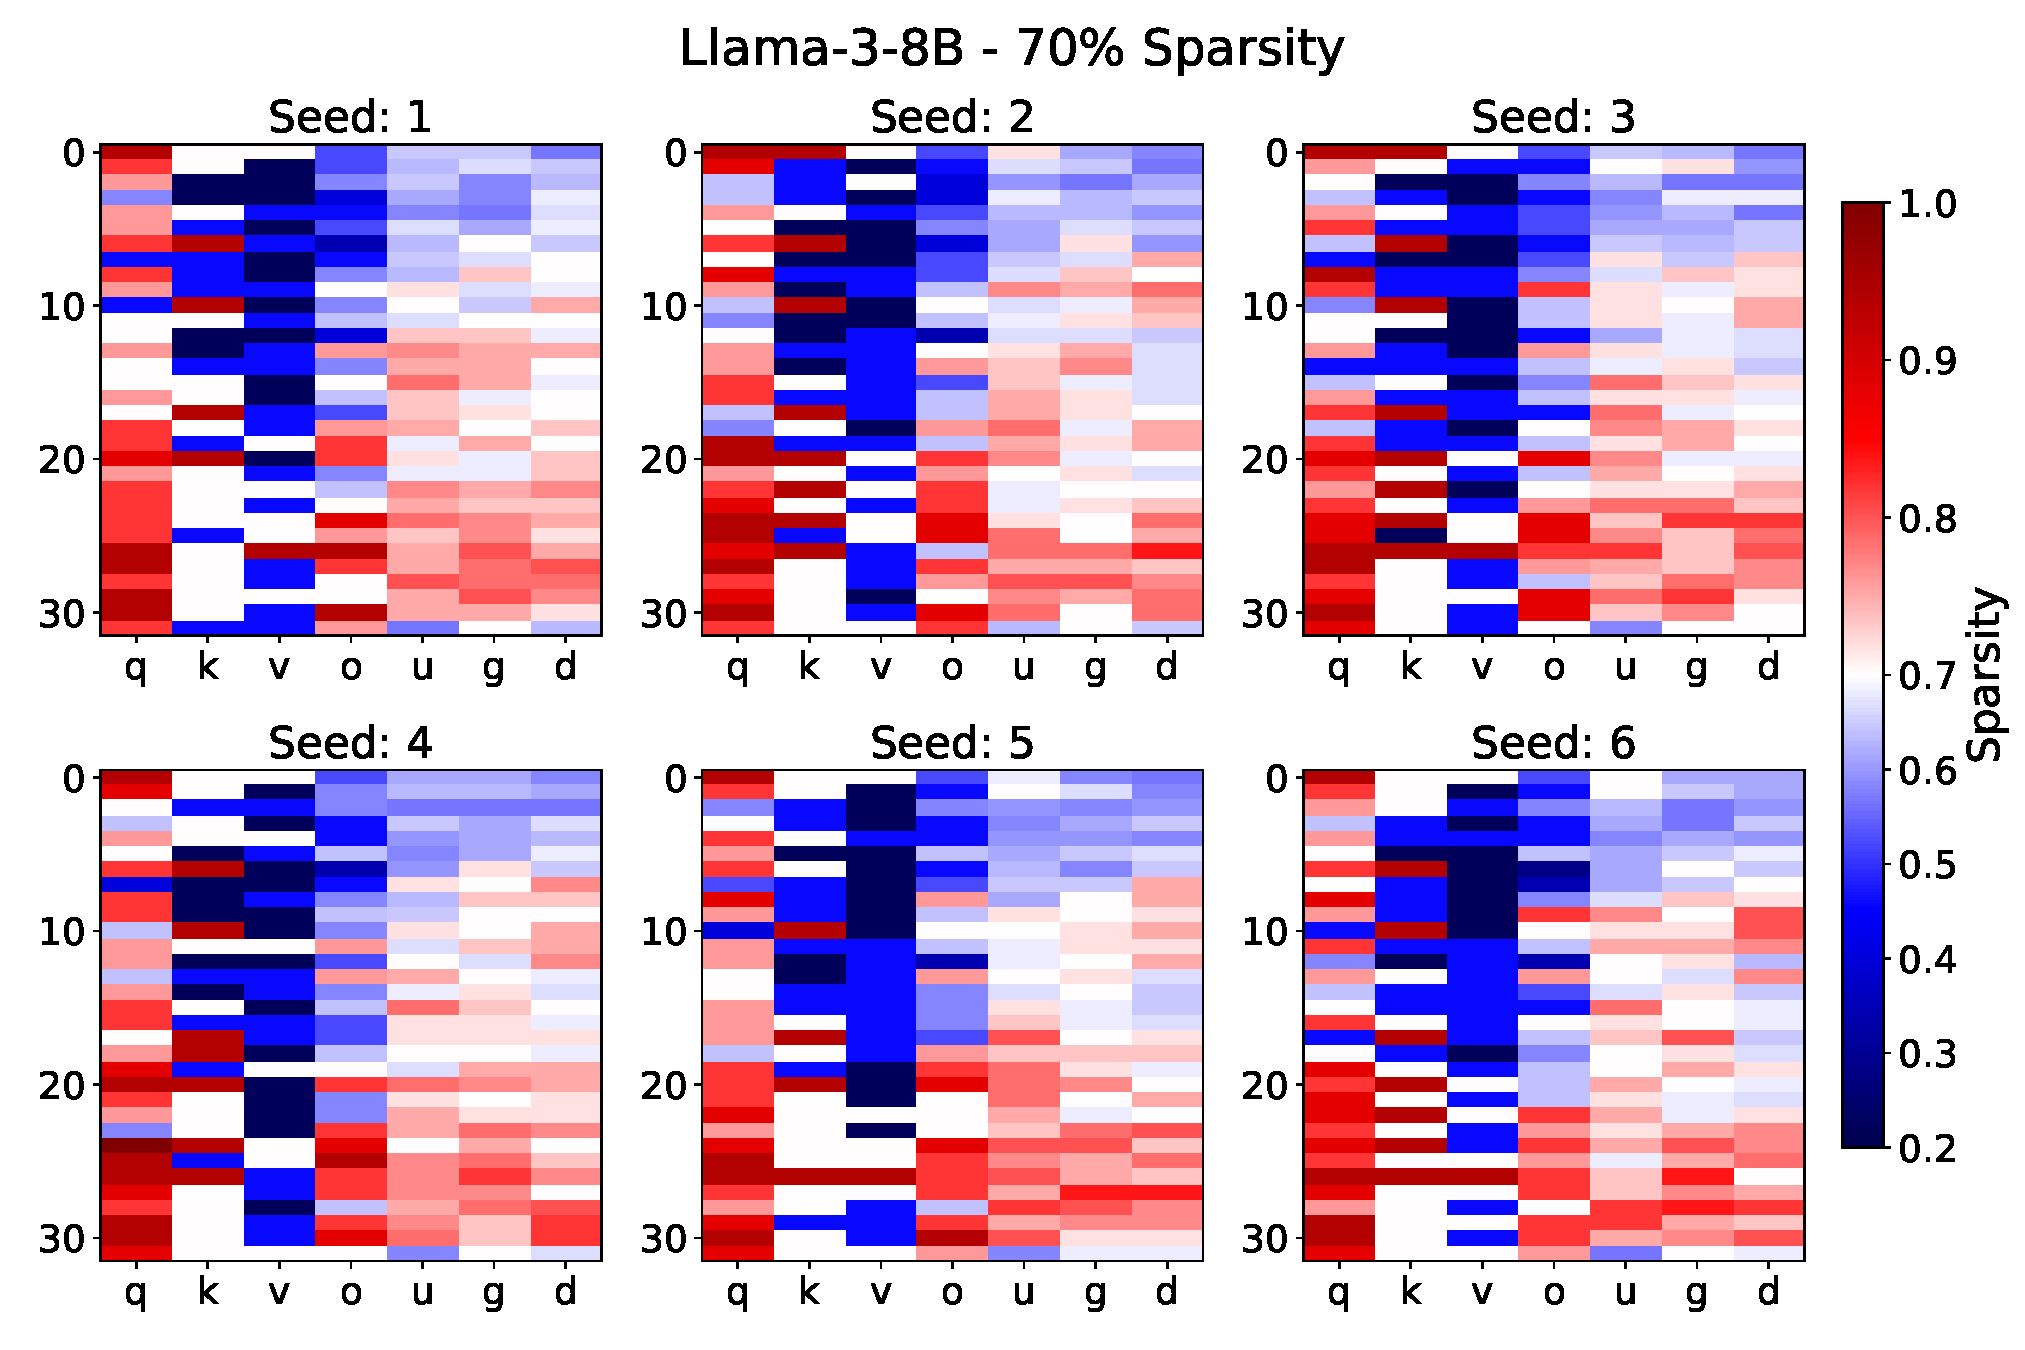
\includegraphics[width=0.92\linewidth]{graphics/Ablations/robustness.pdf}
    \caption{Configurations identified by \methodname{} on Llama-3-8B after 1000 generations show high similarity across different seeds. The y-axis represents the depth of the respective transformer block, while the x-axis denotes the corresponding layer (q: query, k: key, v: value, o: output, u: MLP up, g: MLP gate, d: MLP down).}
    \label{fig:robustness_similarity}
\end{figure}
\begin{figure}[htb]
    \centering
    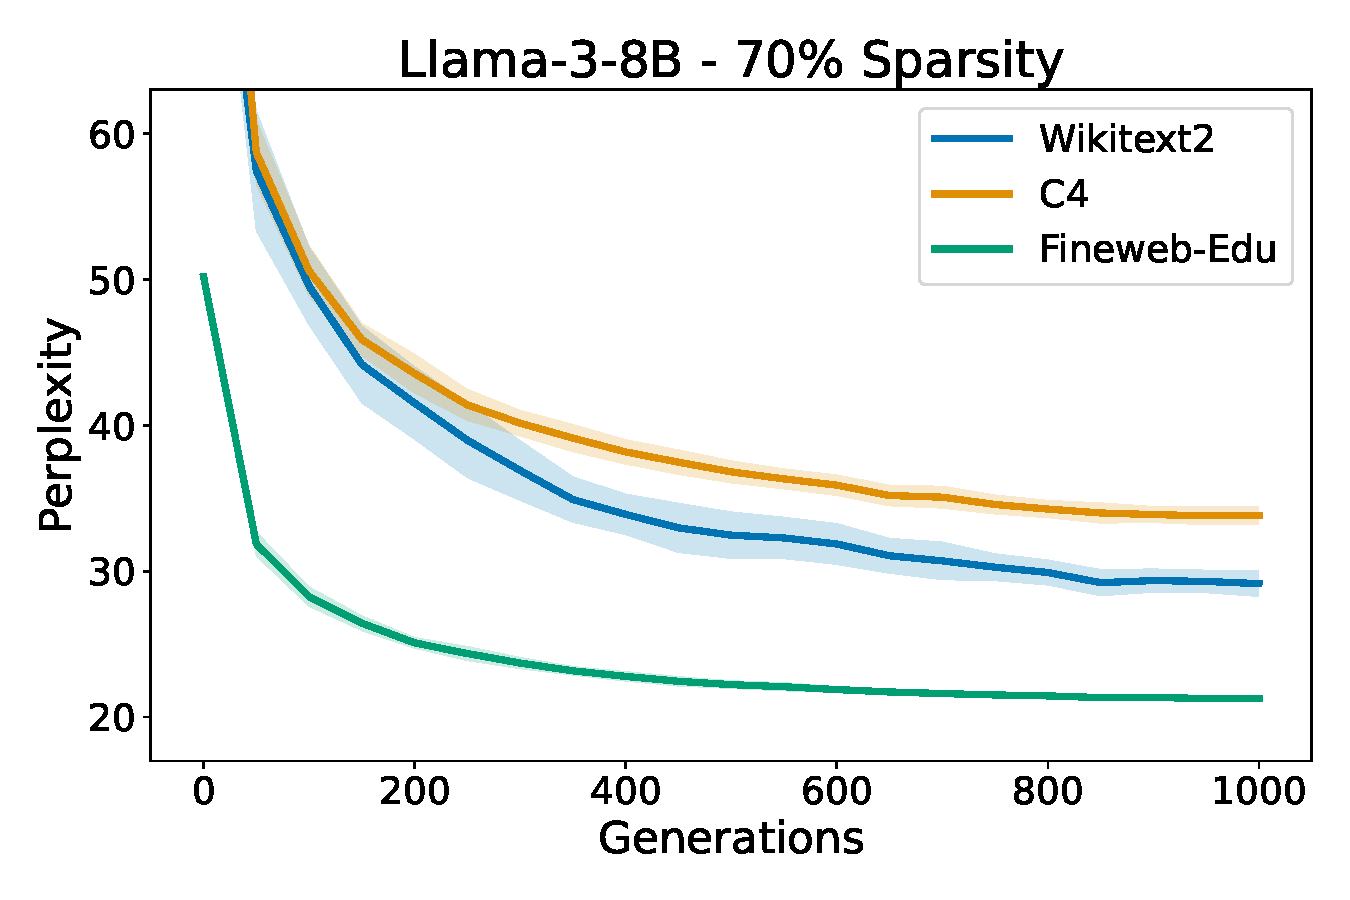
\includegraphics[width=0.55\linewidth]{graphics/Ablations/robustness_convergence.pdf}
    \vspace{-2mm}
    \caption{Convergence behavior of the ``super-fast'' variant across 16 independent runs. The extremely low standard deviation (shaded area) demonstrates the robustness of the method, which suggests that local optima do not pose significant challenges to the search.}
    \label{fig:robustness_convergence}
\end{figure}

\FloatBarrier
\section{Additional Depth Pruning Results}
\subsection{Full Results}
\label{app:depth_full_perplexity}


Here, we present our additional results for depth pruning experiments on Mistral-7B-v0.3 (Table~\ref{tabl:appendix_dropping_mistral}), Llama-2-7B (Table~\ref{tab:llama2-depth-table}),  Llama-3-8B (Table~\ref{tab:llama3-depth-table}), and Llama-3.1-8B (Table~\ref{tab:llama31-depth-table}). Across all levels of sparsities, \methodname{} consistently outperforms previous methods. Additionally, Table~\ref{tabl:appendix_dropping_mistral} includes results where only entire transformer blocks are removed by \methodname{}. This showcases that the significant gains are not primarily due to this relaxation, and that our method performs better than baselines even when dealing with this coarser search space.

\begin{table}[htb]
\footnotesize
\centering
\setlength\tabcolsep{3pt}
\caption{Depth pruning of Llama-2-7B.}
\resizebox{0.58\textwidth}{!}{
\begin{tabular}{c|c|ccc}
\toprule
\textbf{Sparsity} & \textbf{Method} & \textbf{Wiki2$\downarrow$} & \textbf{C4$\downarrow$} & \textbf{FW$\downarrow$} \\ 
\midrule
0\% & Dense & 5.21 & 6.93 & 6.40 \\
\midrule
\multirow{5}{*}{12.5\%}  & EvoPress & \textbf{6.42} & \textbf{8.60} & \textbf{7.54} \\
                         & ShortGPT & 8.86 & 10.78 & 9.30 \\
                         & Cosine Similarity (Window) & 7.53 & 9.82 & 8.51 \\
                         & Weight Subcloning & 9.09 & 11.06 & 9.60 \\
                         & ShortenedLlama & 7.68 & 10.44 & 8.57 \\ 
\midrule
\multirow{5}{*}{25\%}  & EvoPress & \textbf{9.15} & \textbf{11.46} & \textbf{9.69} \\
                       & ShortGPT & 23.41 & 30.30 & 21.16 \\
                       & Cosine Similarity (Window) & 16.60 & 21.04 & 17.37 \\
                       & Weight Subcloning & 23.41 & 30.30 & 21.16 \\
                       & Shortened Llama & 13.86 & 14.08 & 11.81 \\ 
\midrule
\multirow{5}{*}{37.5\%} & EvoPress & \textbf{17.98} & \textbf{18.91} & \textbf{15.53} \\
                        & ShortGPT & 70.94 & 63.51 & 54.07 \\
                        & Cosine Similarity (Window) & 192.07 & 212.60 & 151.10 \\
                        & Weight Subcloning & 70.94 & 63.51 & 54.07 \\
                        & Shortened Llama & 35.37 & 26.07 & 20.37 \\ 
\midrule
\multirow{5}{*}{50\%} & EvoPress & \textbf{48.84} & \textbf{42.29} & \textbf{33.57} \\
                      & ShortGPT & 226.14 & 171.04 & 180.51 \\
                      & Cosine Similarity (Window) & 4570.15 & 2876.83 & 1861.06 \\
                      & Weight Subcloning & 226.14 & 171.04 & 180.51 \\
                      & Shortened Llama & 145.78 & 87.40 & 68.79 \\ 
\bottomrule
\end{tabular}
\label{tab:llama2-depth-table}
}
\end{table}

\begin{table}[htb]
\footnotesize
\centering
\setlength\tabcolsep{3pt}
\caption{Depth pruning of Llama-3-8B.}
\resizebox{0.58\textwidth}{!}{
\begin{tabular}{c|c|ccc}
\toprule
\textbf{Sparsity} & \textbf{Method} & \textbf{Wiki2$\downarrow$} & \textbf{C4$\downarrow$} & \textbf{FW$\downarrow$} \\ 
\midrule
0\% & Dense & 5.54 & 8.80 & 7.62 \\
\midrule
\multirow{5}{*}{12.5\%}  & EvoPress & \textbf{7.72} & \textbf{12.61} & \textbf{10.15} \\
                         & ShortGPT & 13.21 & 19.56 & 14.25 \\
                         & Cosine Similarity (Window) & 9.54 & 14.87 & 11.64 \\
                         & Weight Subcloning & 13.21 & 19.56 & 14.25 \\
                         & Shortened Llama & 9.42 & 15.09 & 11.57 \\ 
\midrule
\multirow{5}{*}{25\%}  & EvoPress & \textbf{13.99} & 22.83 & \textbf{15.84} \\
                       & ShortGPT & 5527.54 & 11589.93 & 2346.13 \\
                       & Cosine Similarity (Window) & 5519.95 & 11629.61 & 2342.91 \\
                       & Weight Subcloning & 5527.54 & 11589.93 & 2346.13 \\
                       & Shortened Llama & 16.59 & \textbf{20.81} & 16.28 \\ 
\midrule
\multirow{5}{*}{37.5\%} & EvoPress & \textbf{27.56} & \textbf{35.70} & \textbf{26.77} \\
                        & ShortGPT & 64281.36 & 13836.12 & 3789.09 \\
                        & Cosine Similarity (Window) & 64627.29 & 13890.14 & 3784.72 \\
                        & Weight Subcloning & 64381.36 & 13836.13 & 3789.09 \\
                        & Shortened Llama & 50.20 & 61.56 & 37.40 \\ 
\midrule
\multirow{5}{*}{50\%} & EvoPress & \textbf{84.99} & \textbf{87.86} & \textbf{66.41} \\
                      & ShortGPT & 1663.97 & 1740.04 & 1588.20 \\
                      & Cosine Similarity (Window) & 2053.19 & 1116.47 & 694.00 \\
                      & Weight Subcloning & 1663.97 & 1740.04 & 1588.20 \\
                      & Shortened Llama & 724.86 & 666.41 & 210.30 \\ 
\bottomrule
\end{tabular}
}
\label{tab:llama3-depth-table}
\end{table}

\begin{table}[htb]
\footnotesize
\centering
\setlength\tabcolsep{3pt}
\caption{Depth pruning of Llama-3.1-8B.}
\resizebox{0.58\textwidth}{!}{
\begin{tabular}{c|c|ccc}
\toprule
\textbf{Sparsity} & \textbf{Method} & \textbf{Wiki2$\downarrow$} & \textbf{C4$\downarrow$} & \textbf{FW$\downarrow$} \\ 
\midrule
0\% & Dense & 5.61 & 8.90 & 7.67 \\
\midrule
\multirow{5}{*}{12.5\%}  & EvoPress & \bf{7.58} & \bf{12.24} & \bf{10.00} \\
                         & ShortGPT & 12.54 & 19.21 & 13.76 \\
                         & Cosine Similarity (Window) & 12.54 & 19.21 & 13.76 \\
                         & Weight Subcloning & 12.54 & 19.21 & 13.76 \\
                         & Shortened Llama & 9.27 & 14.80 & 11.21 \\
\midrule
\multirow{5}{*}{25\%}  & EvoPress & \bf{11.59} & \bf{17.84} & \bf{13.96} \\
                       & ShortGPT & 4278.39 & 6754.92 & 1512.39 \\
                       & Cosine Similarity (Window) & 4278.39 & 6754.92 & 1512.39 \\
                       & Weight Subcloning & 4278.39 & 6754.92 & 1512.39 \\
                       & Shortened Llama & 20.41 & 20.33 & 16.12 \\
\midrule
\multirow{5}{*}{37.5\%} & EvoPress & \bf{24.98} & \bf{35.77} & \bf{25.93} \\
                        & ShortGPT & 123044.19 & 22071.51 & 6059.03 \\
                        & Cosine Similarity (Window) & 123044.19 & 22071.51 & 6059.03 \\
                        & Weight Subcloning & 123044.19 & 22071.51 & 6059.03 \\
                        & Shortened Llama &  41.34 & 43.53 & 31.00 \\
\midrule
\multirow{5}{*}{50\%} & EvoPress & \bf{105.84} & \bf{110.69} & \bf{61.25} \\
                      & ShortGPT & 1630.11 & 1680.21 & 1698.64 \\
                      & Cosine Similarity (Window) & 1881.54 & 1196.63 & 683.24 \\
                      & Weight Subcloning & 1630.11 & 1680.21 & 1698.64 \\
                      & Shortened Llama & 454.96 & 309.42 & 153.96 \\
\bottomrule
\end{tabular}
}
\label{tab:llama31-depth-table}
\end{table}


\begin{table}[htb]
\footnotesize
\centering
\setlength\tabcolsep{3pt}
\caption{Depth pruning of Mistral-7B-v0.3.}
\resizebox{0.58\textwidth}{!}{
\begin{tabular}{c|c|ccc}
\toprule
\textbf{Sparsity} & \textbf{Method} & \textbf{Wiki2$\downarrow$} & \textbf{C4$\downarrow$} & \textbf{FW$\downarrow$} \\ 
\midrule
0\% & Dense & 4.82 & 7.72 & 6.41 \\
\midrule
\multirow{5}{*}{12.5\%}  & EvoPress & \textbf{6.06} & \textbf{9.00} & \textbf{7.42} \\
& EvoPress (Attn.+MLP) & 6.33 & 9.44 & 7.80 \\
                         & ShortGPT & 7.19 & 10.18 & 8.46 \\
                         & Cosine Similarity (Window) & 7.19 & 10.18 & 8.46 \\
                         & Weight Subcloning & 7.19 & 10.18 & 8.46 \\
                         & Shortened Llama & 6.64 & 9.71 & 7.94 \\ 
\midrule
\multirow{5}{*}{25\%}  & EvoPress & \textbf{8.66} & \textbf{12.04} & \textbf{9.92} \\
& EvoPress (Attn.+MLP) & 9.46  & 13.02  & 10.59 \\
                       & ShortGPT & 43.26 & 40.16 & 29.54 \\
                       & Cosine Similarity (Window) & 33.75 & 54.07 & 36.26 \\
                       & Weight Subcloning & 43.26 & 40.16 & 29.54 \\
                       & Shortened Llama & 14.94 & 19.30 & 14.73 \\ 
\midrule
\multirow{5}{*}{37.5\%} & EvoPress & \textbf{17.52} & \textbf{21.60} & \textbf{16.90} \\
& EvoPress (Attn.+MLP) & 21.62  & 25.17 & 18.97  \\
                        & ShortGPT & 2898.98 & 2722.66 & 981.99 \\
                        & Cosine Similarity (Window) & 1034.09 & 2471.86 & 1050.56 \\
                        & Weight Subcloning & 2898.98 & 2722.66 & 981.99 \\
                        & Shortened Llama & 440.20 & 442.09 & 486.15 \\ 
\midrule
\multirow{5}{*}{50\%} & EvoPress & \textbf{61.75} & \textbf{54.15} & \textbf{43.23} \\
& EvoPress (Attn.+MLP) & 108.91  & 99.74 & 69.07 \\
                      & ShortGPT & 2422.72 & 2134.92 & 1083.51 \\
                      & Cosine Similarity (Window) & 3411.47 & 1934.16 & 1740.91 \\
                      & Weight Subcloning & 2422.72 & 2134.92 & 1083.51 \\
                      & Shortened Llama & 5241.76 & 3595.71 & 1953.14 \\ 
\bottomrule
\end{tabular}
\label{tabl:appendix_dropping_mistral}
}
\end{table}

 \FloatBarrier


\subsection{Practical Convergence}
\label{appendix:sec:conv_dropping}
\methodname{} identifies superior compression profiles in a highly efficient manner. Figure~\ref{fig:conv_dropping} displays that the evolutionary search produces better compressed models than previous techniques in a matter of minutes, with full convergence in around half an hour. 

\begin{figure}[htb]
    \centering
    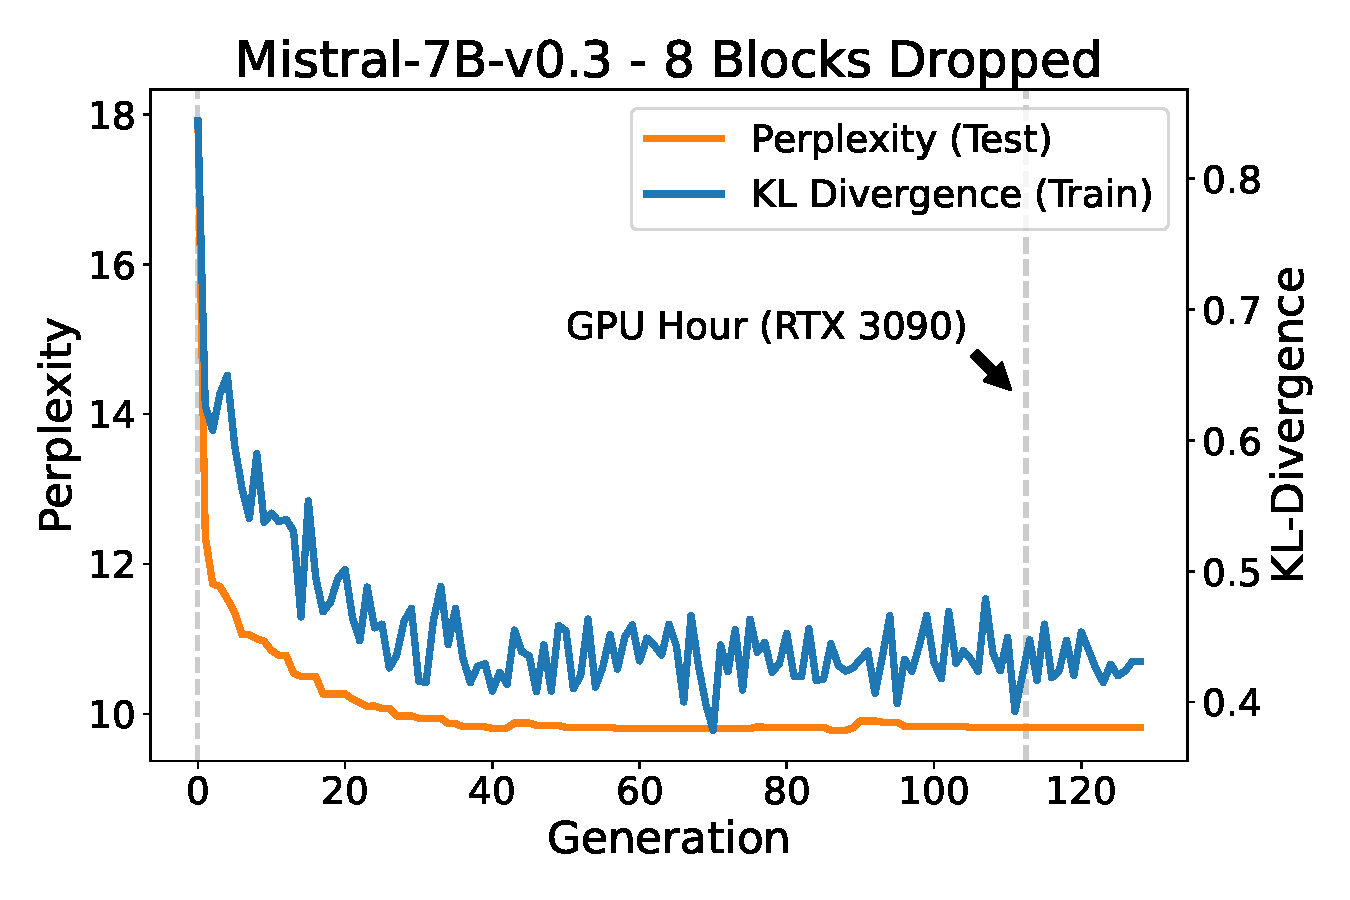
\includegraphics[width=0.48\linewidth]{graphics/Convergence/Convergence_Mistral_8Dropped.pdf}
    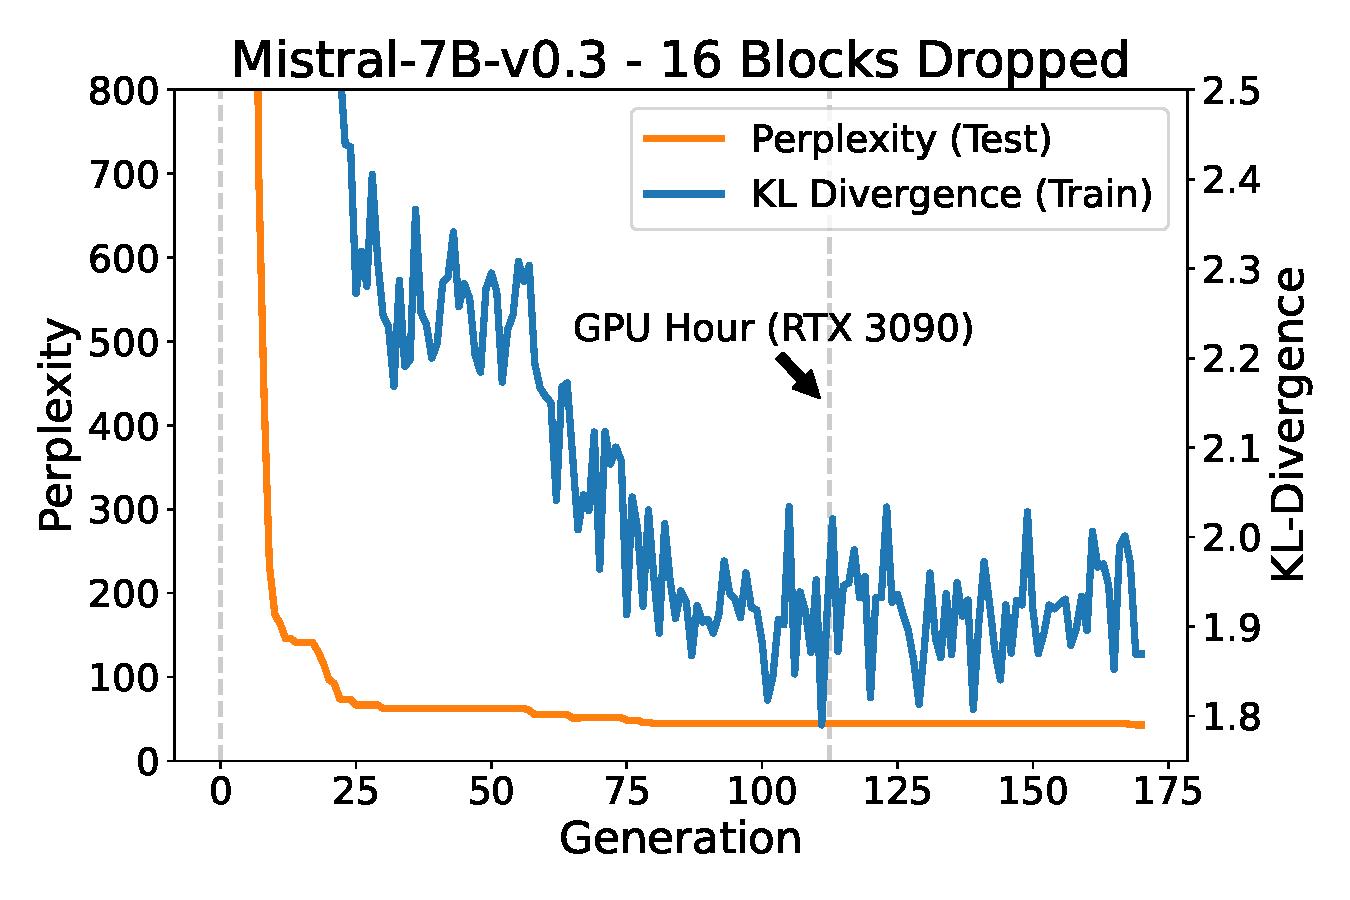
\includegraphics[width=0.48\linewidth]{graphics/Convergence/Convergence_Mistral_16Dropped.pdf}
    \caption{Convergence of \methodname{} when removing 8 transformer blocks (left) and 16 transformer blocks (right) of Mistral-7B-v0.3.} 
    \label{fig:conv_dropping}
\end{figure}

\subsection{Locality of Dropped Blocks}
\label{app:locality_dropped}
Prior research indicates that deeper layers, aside from the final ones, are generally less effective \citep{ineffect_of_deeper, shortgpt}. Figure~\ref{fig:drop_configs} illustrates the optimal removal configurations identified by \methodname{}. For comparison, Table~\ref{tab:appendix_removal_order} displays the removal order of prior scoring methods. While \methodname{} indeed removes some deeper layers across all sparsities, we also observe that certain shallow layers appear to be less important. Notably, a ``two hills'' pattern emerges in many cases, where blocks before and after the midpoint are pruned, yet the central blocks remain intact. Meanwhile, the first two blocks are never pruned. However, in contrast to a heuristic proposed by \citet{llmpruner}, we find that, in some instances, it is effective to prune the final block as well. 

\begin{figure}[htb]
    \centering
    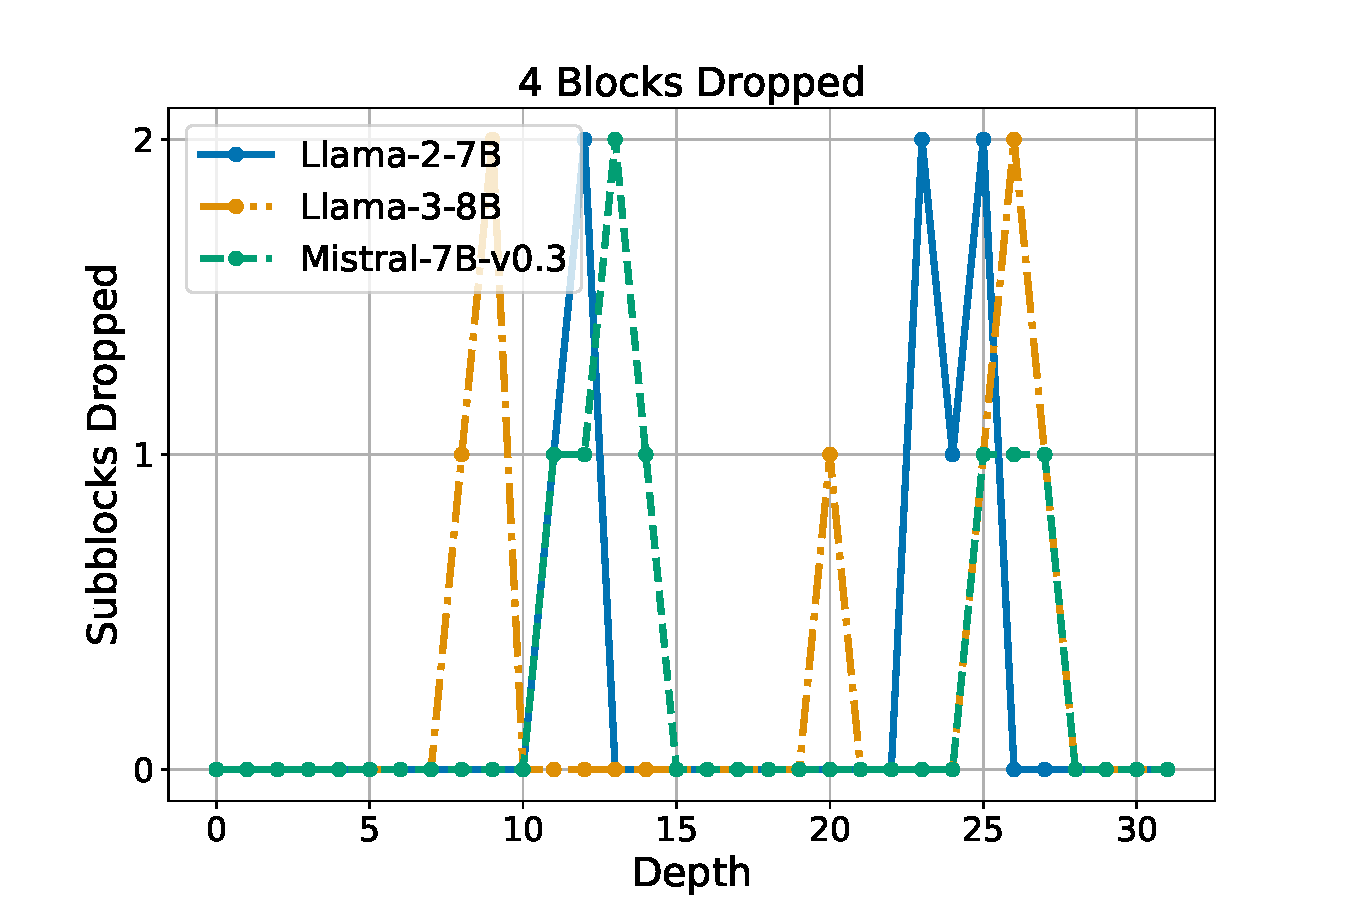
\includegraphics[width=0.46\linewidth]{graphics/BlockDroppingAppendix/running_average_4.pdf}
    \hspace{0.02\linewidth}
    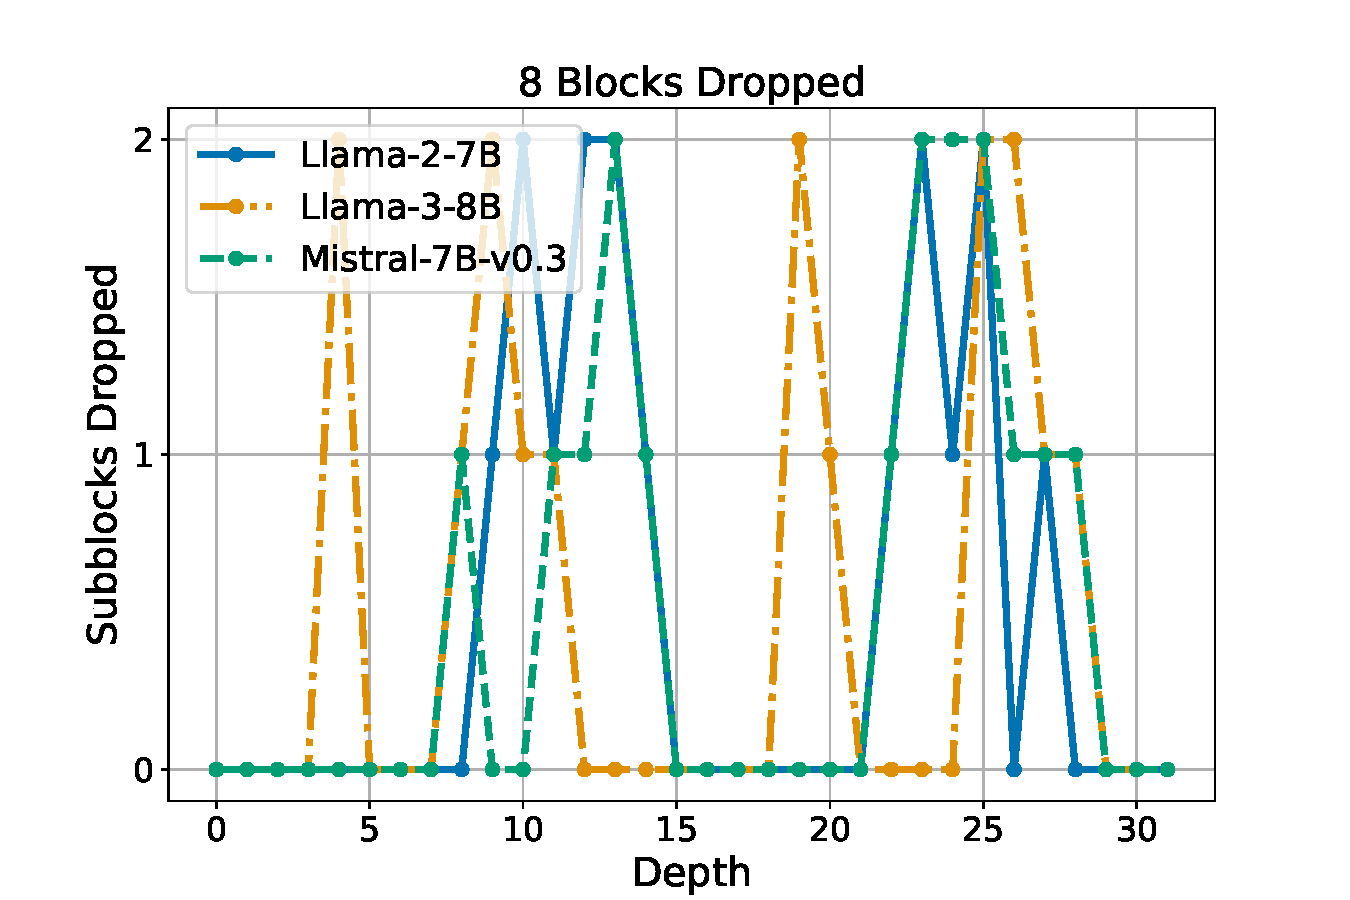
\includegraphics[width=0.46\linewidth]{graphics/BlockDroppingAppendix/running_average_8.pdf}

    \vspace{0.2em}
    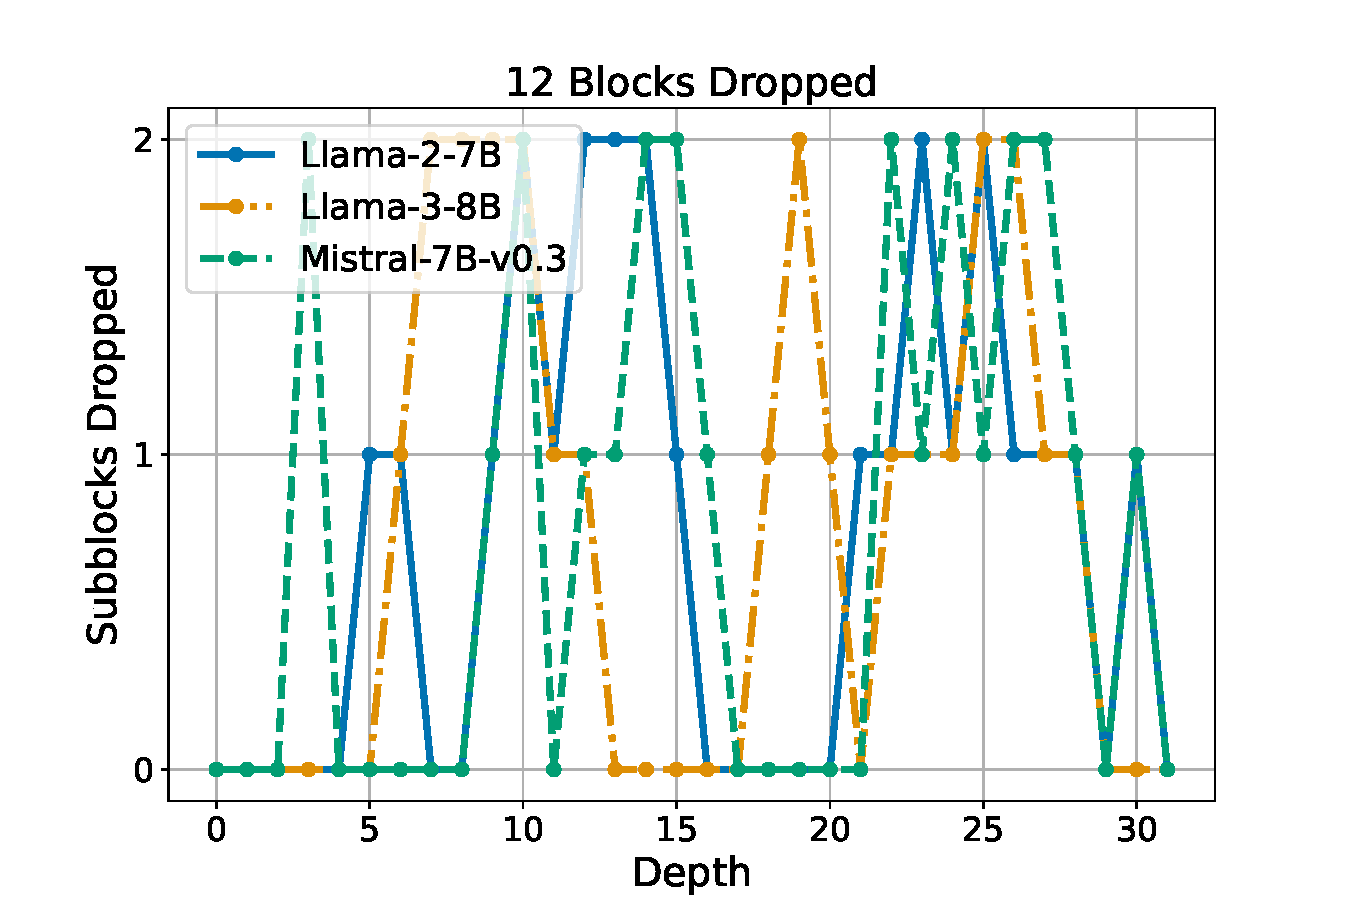
\includegraphics[width=0.46\linewidth]{graphics/BlockDroppingAppendix/running_average_12.pdf}
    \hspace{0.02\linewidth}
    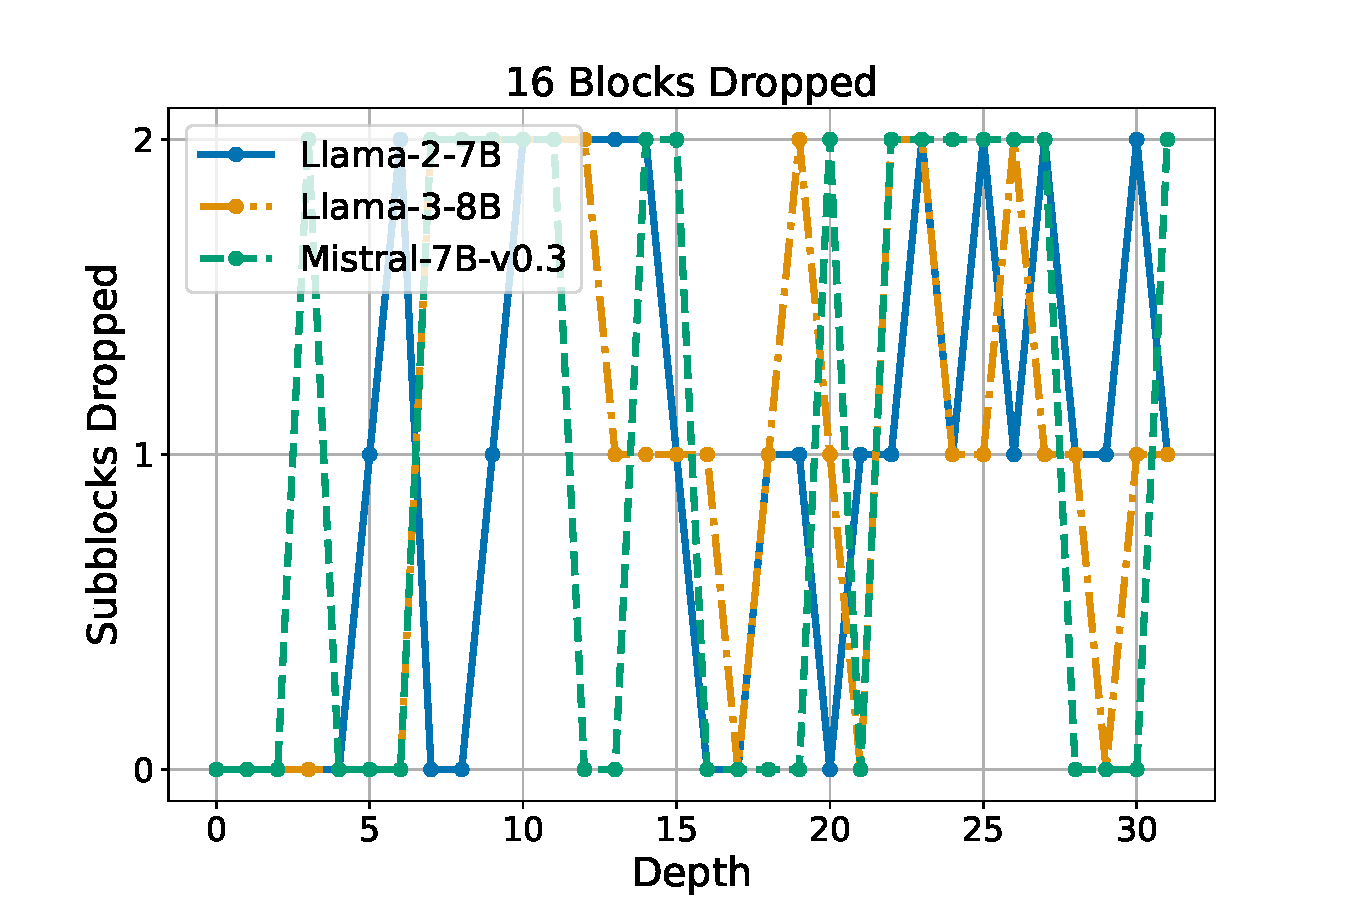
\includegraphics[width=0.46\linewidth]{graphics/BlockDroppingAppendix/running_average_16.pdf}

    \caption{Optimal removal configurations identified by \methodname{} for different models.}
    \label{fig:drop_configs}
\end{figure}

\begin{table}[htb]
\footnotesize
\centering
\setlength\tabcolsep{3pt}
\caption{First 16 blocks in removal order of ShortGPT, Weight Subcloning and Shortened Llama on different models.}
\resizebox{0.8\textwidth}{!}{
\begin{tabular}{c|c|c}
\toprule
\textbf{Model} & \textbf{Method} & \textbf{Removal Order (Left to Right)}  \\ 
\midrule
\multirow{3}{*}{Mistral-7B-v0.3} & ShortGPT & 26, 25, 24, 27, 23, 22, 28, 30, 21, 29, 20, 19, 13, 17, 18, 12  \\
                    & Weight Subcloning & 26, 25, 24, 27, 23, 28, 22, 30, 21, 29, 20, 19, 13, 17, 12, 18 \\
                    & Shortened Llama & 10, 12, 13, 11, 08, 09, 14, 15, 07, 06, 04, 27, 24, 16, 25, 05 \\
\midrule
\multirow{3}{*}{Llama-2-7B} & ShortGPT & 27, 25, 26, 28, 29, 24, 23, 22, 21, 30, 20, 19, 18, 17, 15, 14 \\
                    & Weight Subcloning & 27, 25, 28, 29, 26, 24, 23, 22, 21, 19, 30, 20, 18, 17, 14, 15  \\
                    & Shortened Llama & 11, 12, 08, 09, 10, 06, 24, 25, 07, 14, 23, 13, 22, 21, 15, 27 \\
\midrule
\multirow{3}{*}{Llama-3-8B} & ShortGPT & 25, 26, 27, 24, 28, 23, 22, 29, 20, 21, 19, 18, 30, 17, 16, 11 \\
                    & Weight Subcloning & 25, 27, 26, 24, 28, 23, 22, 29, 20, 21, 19, 18, 30, 17, 16, 11  \\
                    & Shortened Llama & 10, 08, 09, 11, 26, 25, 12, 22, 24, 23, 14, 13, 28, 06, 19, 21 \\
\midrule
\multirow{3}{*}{Llama-3.1-8B} & ShortGPT &  25, 26, 24, 27, 23, 28, 22, 29, 20, 21, 19, 18, 17, 30, 16, 10 \\
                    & Weight Subcloning &  25, 27, 26, 24, 28, 23, 22, 29, 20, 21, 19, 18, 30, 17, 16, 10 \\
                    & Shortened Llama &  10, 09, 11, 08, 26, 25, 12, 24, 22, 23, 14, 28, 06, 13, 19, 21\\
\bottomrule
\end{tabular}
}
\label{tab:appendix_removal_order}
\end{table}


\FloatBarrier

\subsection{Correlation of Scores with Perplexity}
\looseness=-1
In this experiment, we first calculated the cosine similarity and squared error for each block by comparing activations before and after the block. Next, we randomly removed subsets of blocks (excluding the first and last two) and for each configuration, computed the average cosine similarity and squared error. The results are shown in Figure~\ref{fig:correlation_scores_with_ppl}. Initially, the average squared error exhibited a negative correlation, as the $\ell_2$-norm of the activations increased with depth. This led to configurations with early blocks removed having small average error. To mitigate this, we normalized the activations prior to computing the squared error, which significantly improved the correlation, resulting in performance comparable to cosine similarity. However, as sparsity increased, the correlation degraded significantly for both methods, offering insight into why removal techniques based on scoring fail even at moderate levels of sparsity. Meanwhile, when removing only a small number of blocks, the average perplexity when removing each block separatly is a strong predictor of the performance after removing an entire set of blocks, as depicted in Figure~\ref{fig:correlation_ppl_with_ppl}. We conclude that error monotonicity holds at smaller compression levels, but decays rapidly at medium sparsity. The experiments were done using 131,072 tokens from the Fineweb-Edu calibration dataset.

\begin{figure}

    \caption{Effect of removing random subsets of $2$, $4$, and $6$ blocks for Llama-3-8B. The x-axis depicts the average perplexity when removing each block separately, while the y-axis depicts the perplexity after removing the entire set of blocks. Error monotonicity holds for smaller compression levels, but decays with increasing sparsity.}
    \centering

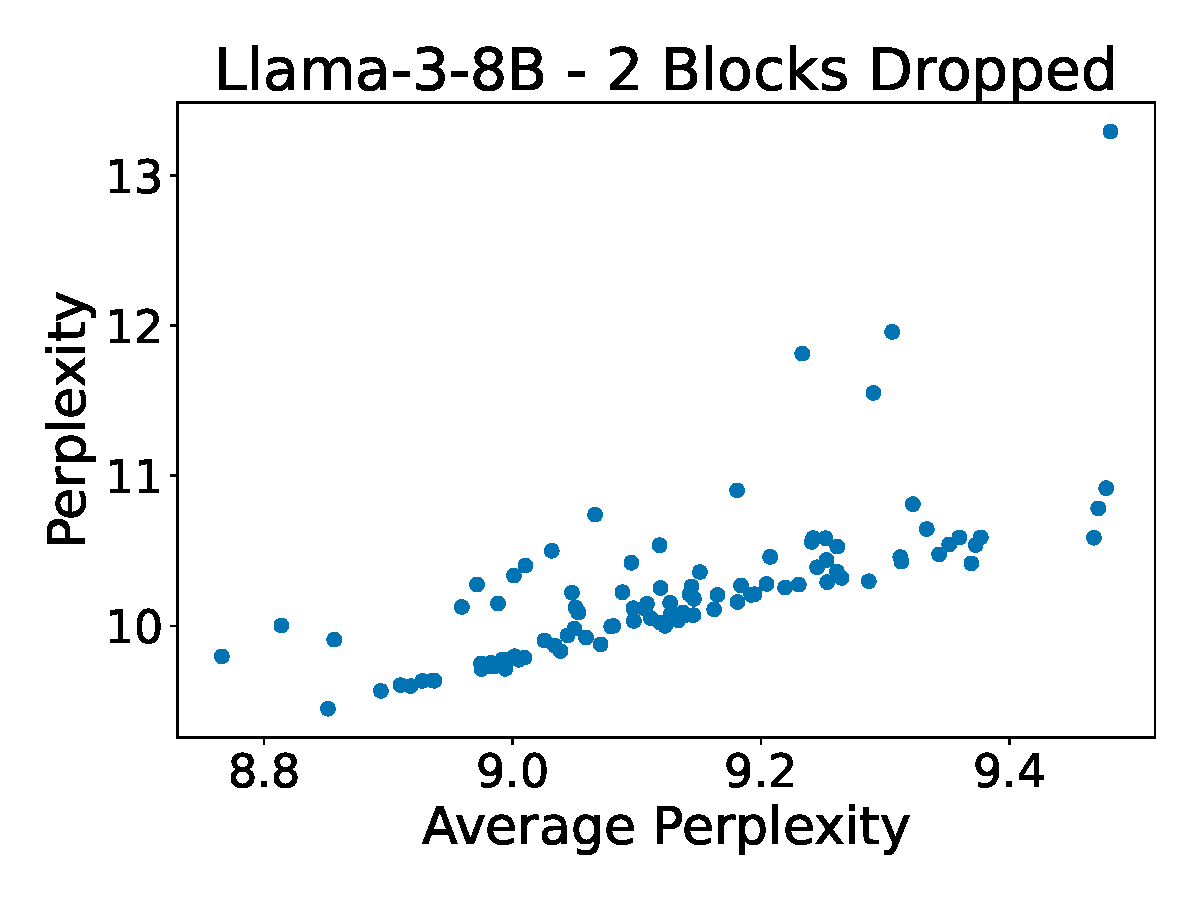
\includegraphics[width=0.32\linewidth]{graphics/BlockDroppingAppendix/linearity_2.pdf}
\hfill
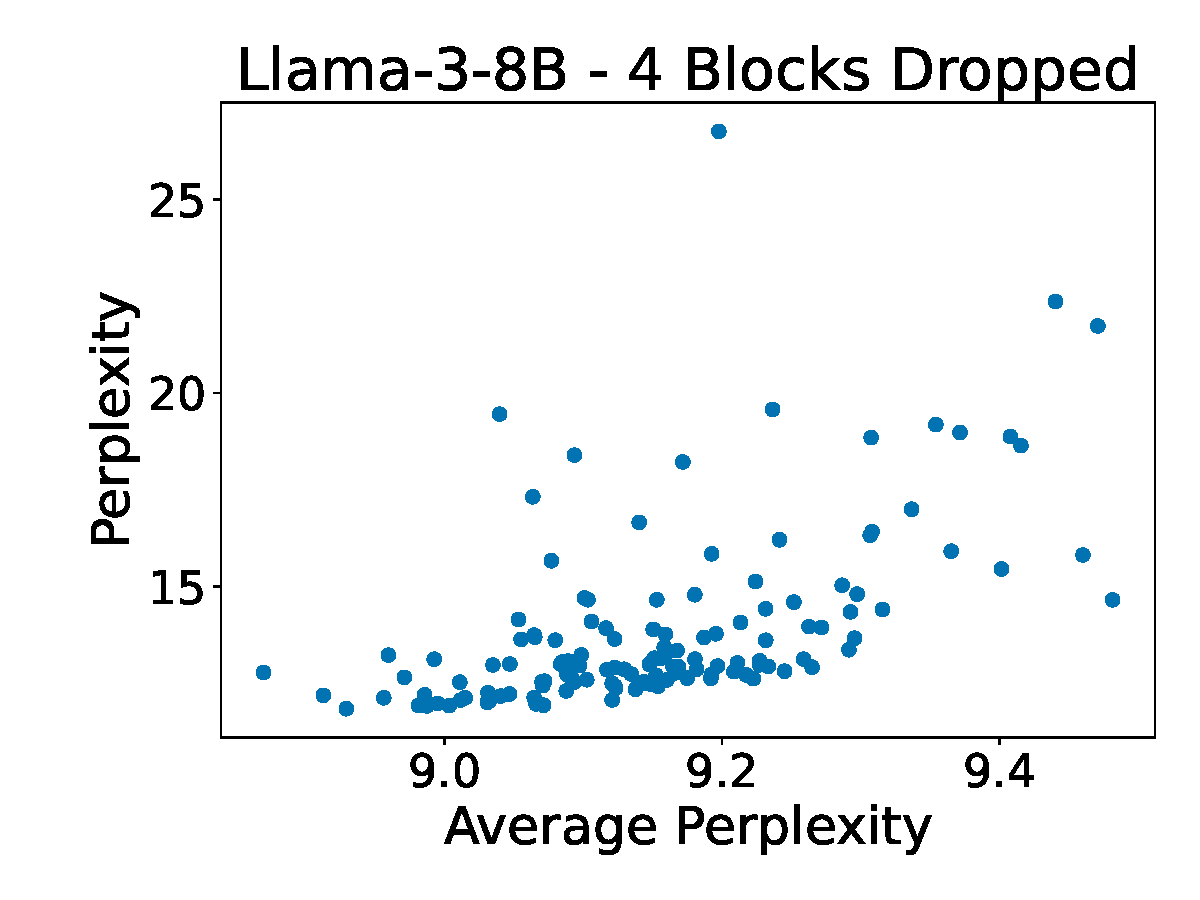
\includegraphics[width=0.32\linewidth]{graphics/BlockDroppingAppendix/linearity_4.pdf}
\hfill
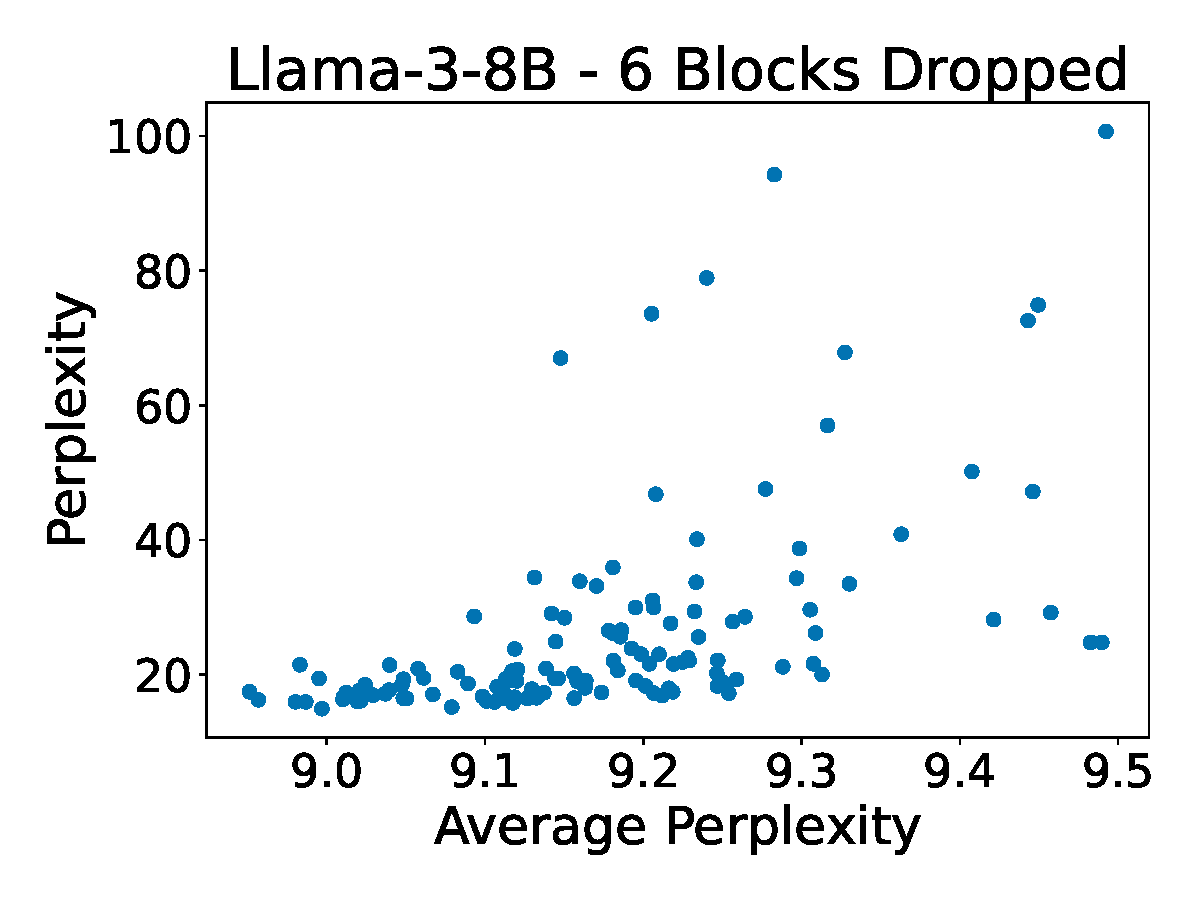
\includegraphics[width=0.32\linewidth]{graphics/BlockDroppingAppendix/linearity_6.pdf}
    \label{fig:correlation_ppl_with_ppl}
\end{figure}
\begin{figure}[htb]
\centering

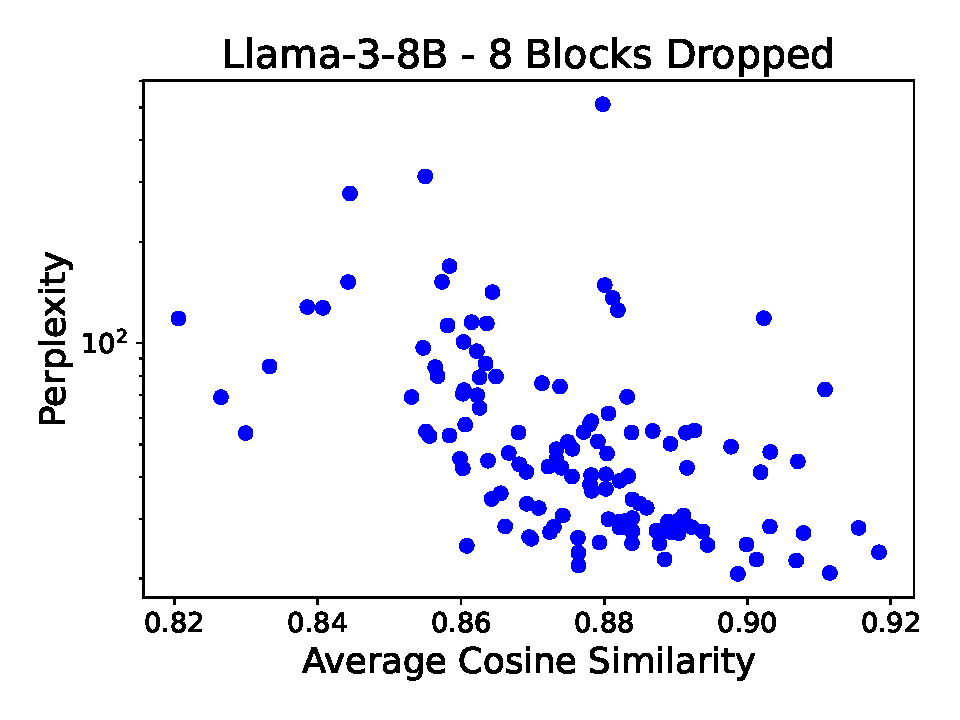
\includegraphics[width=0.32\linewidth]{graphics/BlockDroppingAppendix/CosSimVsPpl_8.pdf}
\hfill
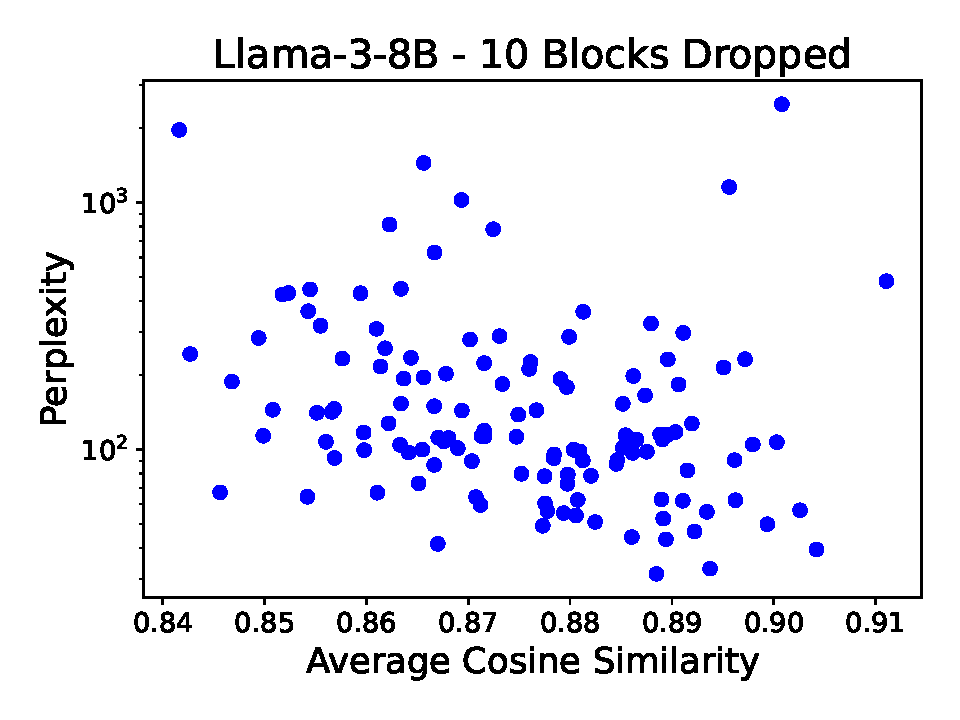
\includegraphics[width=0.32\linewidth]{graphics/BlockDroppingAppendix/CosSimVsPpl_10.pdf}
\hfill
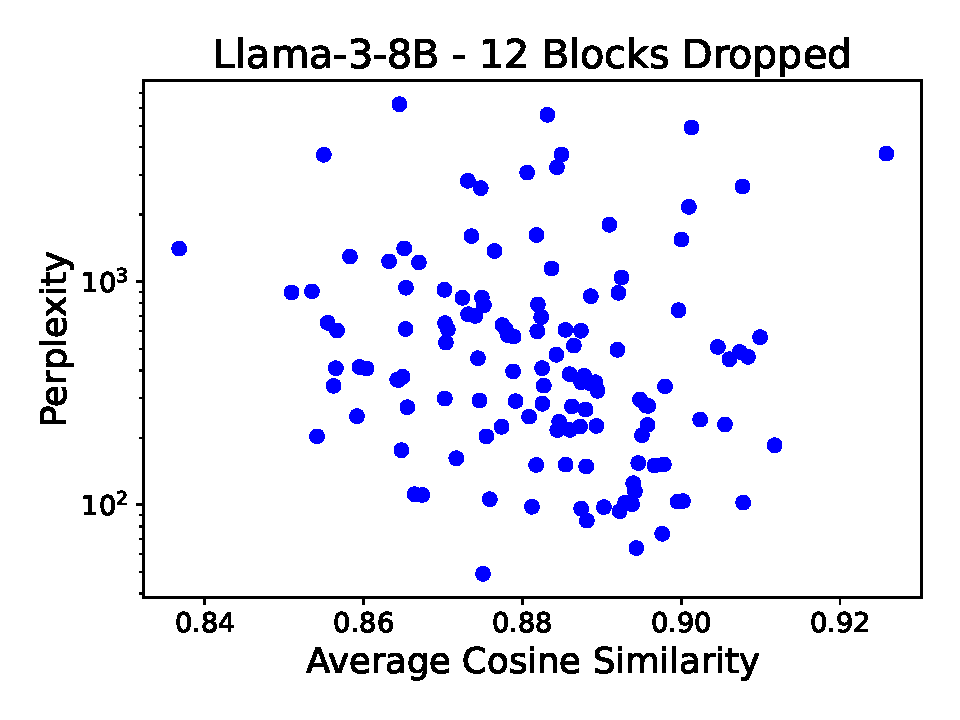
\includegraphics[width=0.32\linewidth]{graphics/BlockDroppingAppendix/CosSimVsPpl_12.pdf}

\vspace{1em}

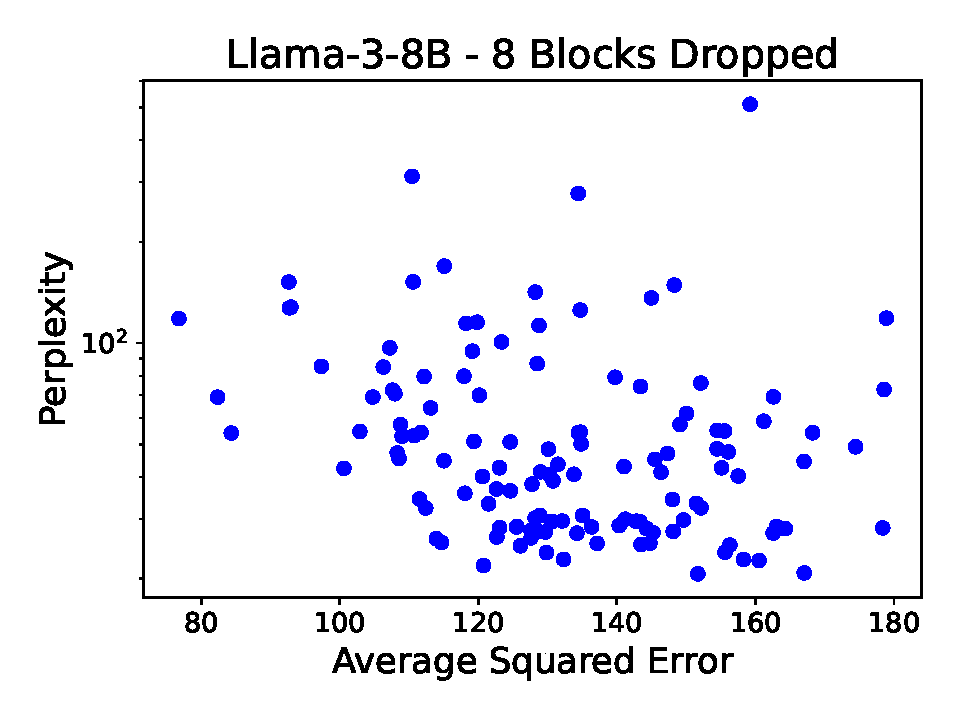
\includegraphics[width=0.32\linewidth]{graphics/BlockDroppingAppendix/l2VsPpl_8.pdf}
\hfill
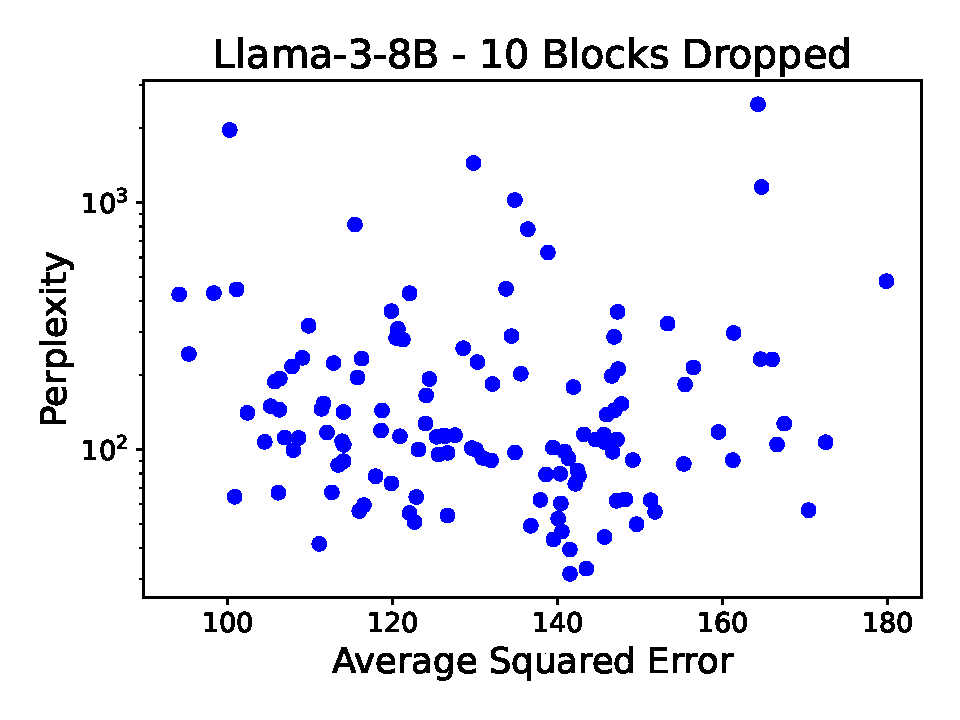
\includegraphics[width=0.32\linewidth]{graphics/BlockDroppingAppendix/l2VsPpl_10.pdf}
\hfill
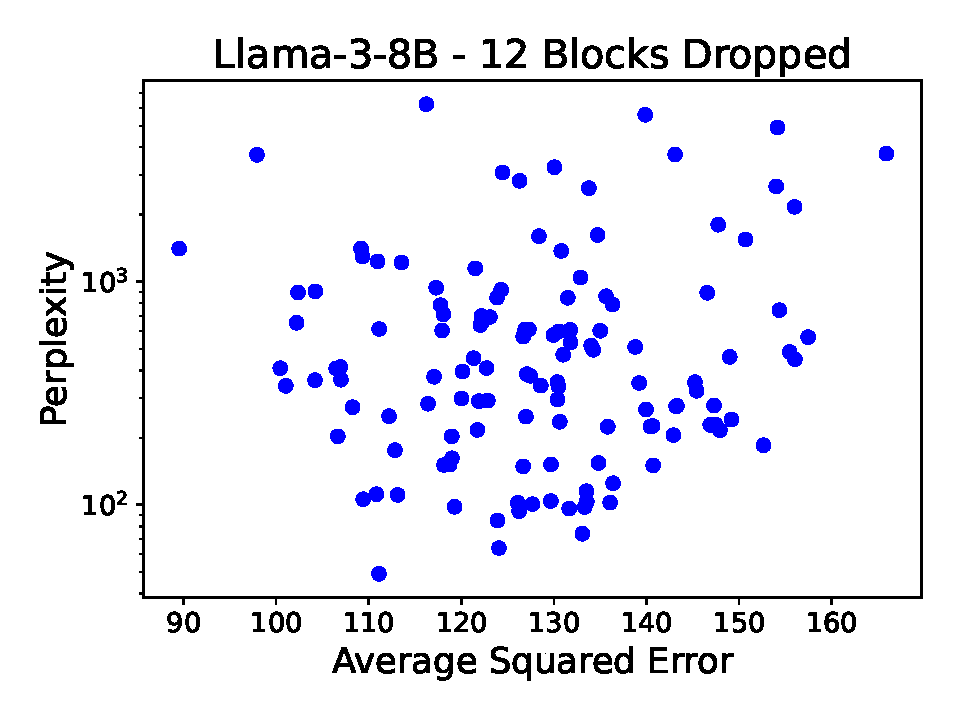
\includegraphics[width=0.32\linewidth]{graphics/BlockDroppingAppendix/l2VsPpl_12.pdf}

\vspace{1em}

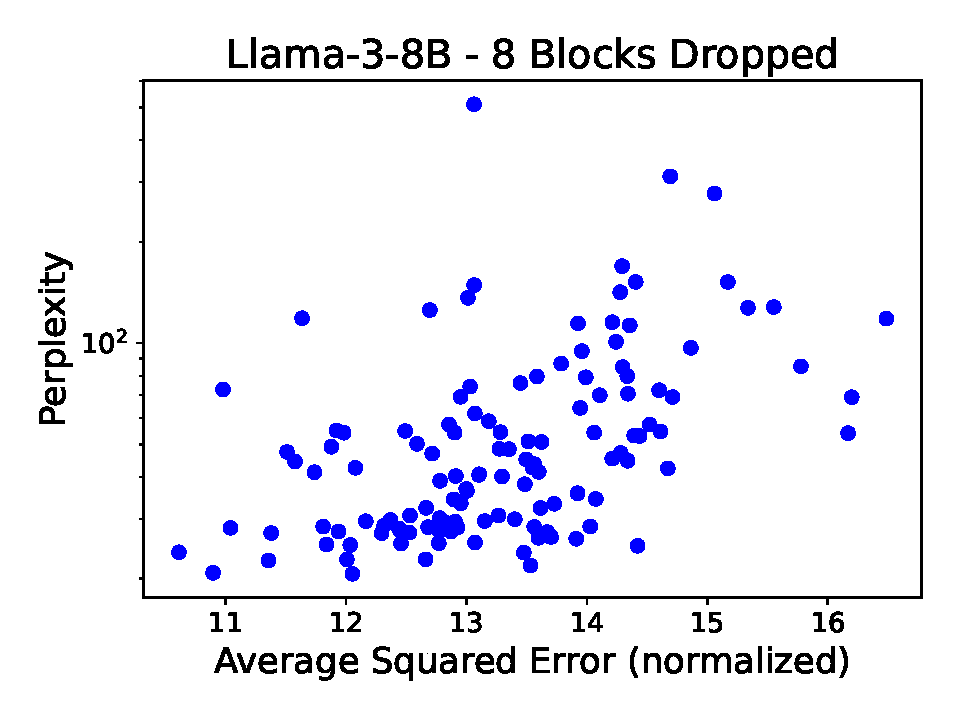
\includegraphics[width=0.32\linewidth]{graphics/BlockDroppingAppendix/l2NormVsPpl_8.pdf}
\hfill
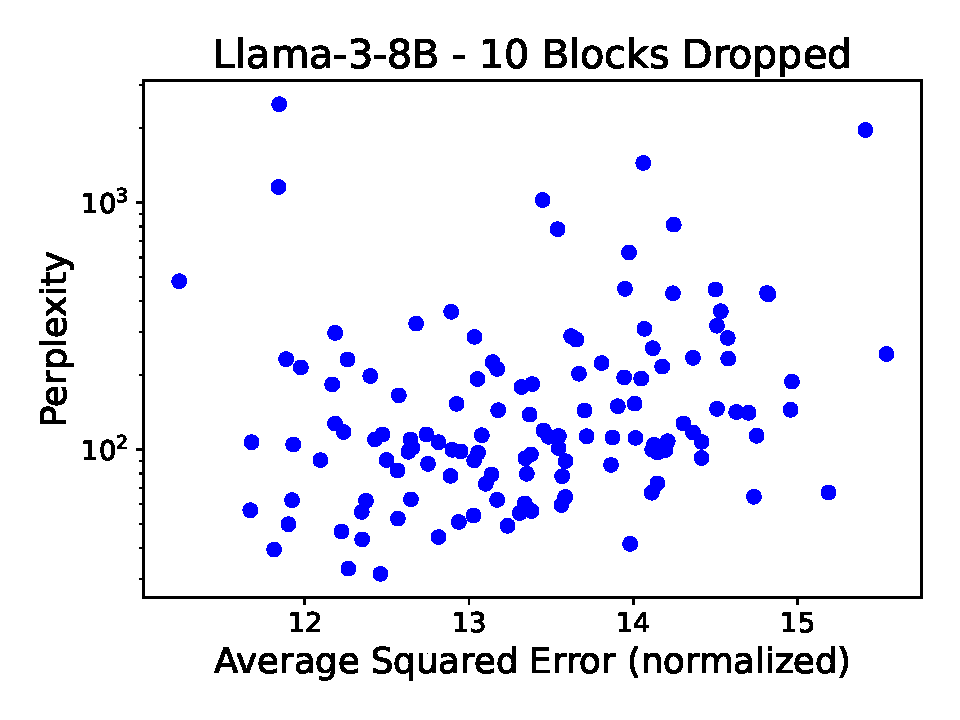
\includegraphics[width=0.32\linewidth]{graphics/BlockDroppingAppendix/l2NormVsPpl_10.pdf}
\hfill
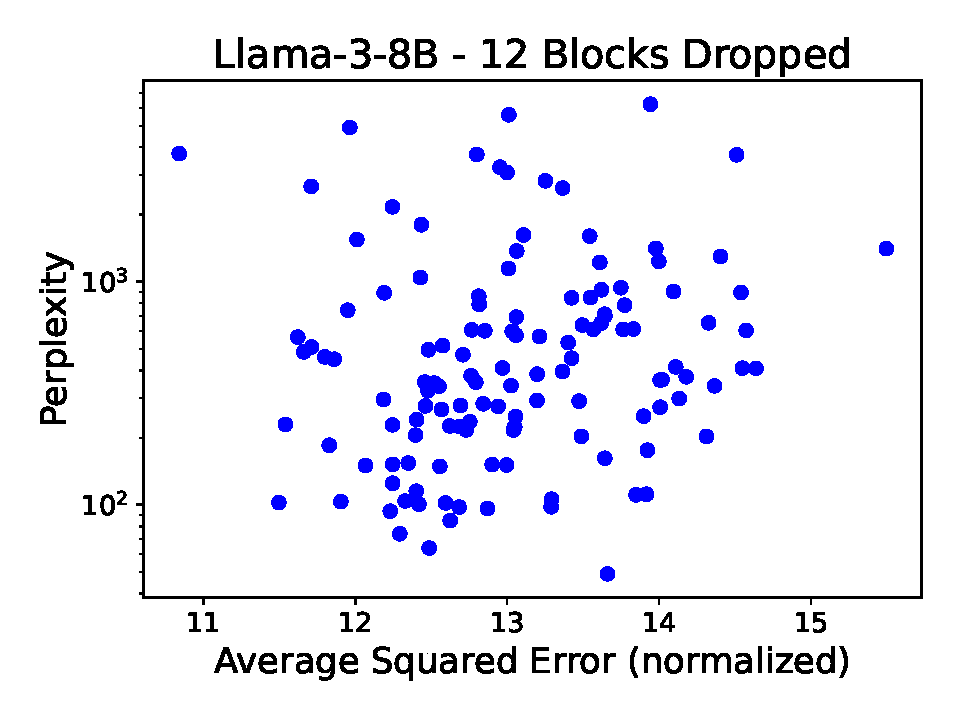
\includegraphics[width=0.32\linewidth]{graphics/BlockDroppingAppendix/l2NormVsPpl_12.pdf}

\caption{Effect of removing random subsets of $8$, $10$, and $12$ blocks for Llama-3-8B. The x-axis depicts the average cosine similarity (first row), average squared error (second row), and the average squared error after normalization (third row) when removing each block separately, while the y-axis depicts the perplexity after removing the entire set of blocks. Error monotonicity breaks at medium sparsity rates, providing an explanation for the failure of scoring-based methods at these sparsity levels.}
\label{fig:correlation_scores_with_ppl}
\end{figure}


\FloatBarrier

\section{Additional Unstructured Sparsity Results}
\subsection{50\% and 60\% Sparsity}
In the main text, we focused on results at 70\% sparsity, where the performance differences are more pronounced. However, since 50\% and 60\% sparsity levels are more practical and frequently referenced in the literature, we present the corresponding results in Tables~\ref{tab:sparsity_50} and~\ref{tab:sparsity_60}. We have also included Llama-2-7B in these tables for legacy purposes. Even at these lower sparsity levels, \methodname{} demonstrates significant improvements over uniform sparsity and consistently outperforms OWL.

\begin{table}[htb]
\footnotesize
\centering
\setlength\tabcolsep{3pt}
\caption{Performance of various sparsity profiles at 50\% sparsity.}\label{tab:sparsity_50}
\resizebox{0.75\textwidth}{!}{
\begin{tabular}{c|c|cc|ccccc|c}
    \toprule
    \bf{Model} & \bf{Method} & \bf{Wiki2$\downarrow$} & \bf{C4$\downarrow$} & \bf{ArcC$\uparrow$} & \bf{ArcE$\uparrow$} & \bf{HS$\uparrow$} &   \bf{PiQA$\uparrow$} & \bf{WG$\uparrow$} & \bf{Avg$\uparrow$} \\
    \midrule
    \multirow{5}{*}{Mistral-7B-v0.3}  & Dense 
    & 4.82 & 7.72 & 48.9 & 79.6 & 60.9 & 80.3 & 73.9 & 68.7 \\
    \cmidrule{2-10}
    & Uniform & 5.68 & 8.93 & 43.7 & 76.7 & 55.7 & 78.4 & 71.0 & 65.1 \\
    & OWL & 5.69 & 8.94 & 43.9 & 76.9 & 55.4 & 78.5 & 70.3 & 65.0 \\
    & EvoPress & \bf{5.49} & \bf{8.70} & 45.7 & 77.3 & 56.5 & 78.9 & 71.2 & \bf{65.9} \\
    \midrule
    \multirow{5}{*}{Llama-2-7B} & Dense
    & 5.12 & 6.93 & 43.4 & 76.3 & 57.1 & 78.1 & 69.0 & 64.8 \\
    \cmidrule{2-10}
    & Uniform & 6.40 & 8.87 & 41.3 & 73.4 & 52.8 & 75.7 & 68.8 & 62.4 \\
    & OWL & 6.38 & 8.77 & 41.1 & 73.2 & 53.2 & 76.5 & 70.2 & 62.9 \\
    & EvoPress &  \bf{6.22} &  \bf{8.52} & 41.5 & 74.2 & 54.0 & 76.7 & 69.6 &  \bf{63.2} \\
    \midrule
    \multirow{5}{*}{Llama-3-8B} & Dense
    & 5.54 & 7.10 & 50.4 & 80.1 & 60.2 & 79.7 & 72.6 & 68.6 \\
    \cmidrule{2-10}
    & Uniform & 8.05 & 13.07 & 43.6 & 75.7 & 54.2 & 76.1 & 71.7 & 64.3 \\
    & OWL & 8.13 & 13.12 & 43.8 & 75.8 & 54.0 & 75.7 & 72.2 & 64.3 \\
    & EvoPress &  \bf{7.63} &  \bf{12.53} & 43.9 & 77.5 & 54.5 & 76.8 & 72.2 &  \bf{65.0} \\
    \midrule
    \multirow{5}{*}{Llama-3.1-8B} 
    & Dense & 5.61 & 8.90 & 51.2 & 81.4 & 60.0 & 80.1 & 73.9 & 69.3 \\
    \cmidrule{2-10}
    & Uniform & 8.06 & 13.03 & 44.5 & 76.7 & 54.0 & 76.7 & 71.5 & 64.7 \\
    & OWL &  8.02 & 12.99 & 44.2 & 76.5 & 53.8 & 76.8 & 72.5 & 64.8 \\
    & EvoPress & \bf{7.51} & \bf{12.31} & 46.6 & 77.7 & 54.9 & 77.6 & 71.7 & \bf{65.7} \\
    \bottomrule
\end{tabular}
}
\end{table}
\begin{table}[htb]
\footnotesize
\centering
\setlength\tabcolsep{3pt}
\caption{Performance of various sparsity profiles at 60\% sparsity.}\label{tab:sparsity_60}
\resizebox{0.75\textwidth}{!}{
\begin{tabular}{c|c|cc|ccccc|c}
    \toprule
    \bf{Model} & \bf{Method} & \bf{Wiki2$\downarrow$} & \bf{C4$\downarrow$} & \bf{ArcC$\uparrow$} & \bf{ArcE$\uparrow$} & \bf{HS$\uparrow$} & \bf{PiQA$\uparrow$} & \bf{WG$\uparrow$} & \bf{Avg$\uparrow$} \\
    \midrule
    \multirow{5}{*}{Mistral-7B-v0.3}  & Dense 
    & 4.82 & 7.72 & 48.9 & 79.6 & 60.9 & 80.3 & 73.9 & 68.7 \\
    \cmidrule{2-10}
    & Uniform & 7.78 & 11.86 & 38.0 & 72.3 & 49.4 & 75.0 & 69.3 & 60.9 \\
    & OWL & 7.50 & 11.34 & 38.5 & 71.9 & 49.6 & 75.1 & 70.2 & 61.1 \\
    & EvoPress & \bf{7.08} & \bf{10.27} & 40.5 & 72.8 & 51.9 & 76.9 & 68.8 & \bf{62.2} \\
    \midrule
    \multirow{5}{*}{Llama-2-7B} & Dense
    & 5.12 & 6.93 & 43.4 & 76.3 & 57.1 & 78.1 & 69.0 & 64.8 \\
    \cmidrule{2-10}
    & Uniform & 9.3 & 12.37 & 35.8 & 69.5 & 45.9 & 72.4 & 65.9 & 57.9 \\
    & OWL & 8.35 & 11.00 & 36.0 & 69.1 & 47.5 & 73.2 & 66.2 & 58.4 \\
    & EvoPress & \bf{8.21} & \bf{10.34} & 37.1 & 70.6 & 49.3 & 74.4 & 67.6 & \bf{59.8} \\
    \midrule
    \multirow{5}{*}{Llama-3-8B} & Dense
    & 5.54 & 7.10 & 50.4 & 80.1 & 60.2 & 79.7 & 72.6 & 68.6 \\
    \cmidrule{2-10}
    & Uniform & 13.86 & 21.43 & 35.2 & 69.7 & 45.6 & 72.2 & 68.0 & 58.2 \\
    & OWL & 12.37 & 18.53 & 38.0 & 70.3 & 47.7 & 72.1 & 68.5 & 59.3 \\
    & EvoPress & \bf{11.02} & \bf{16.37} & 39.0 & 71.9 & 48.6 & 74.0 & 69.1 & \bf{60.5} \\
    \midrule
     \multirow{5}{*}{Llama-3.1-8B} 
    & Dense & 5.61 & 8.90 & 51.2 & 81.4 & 60.0 & 80.1 & 73.9 & 69.3 \\
    \cmidrule{2-10}
    & Uniform & 13.43 & 21.46 & 36.4 & 69.7 & 46.2 & 72.3 & 67.7 & 58.5 \\
    & OWL &  12.08 & 18.25 & 38.9 & 71.1 & 47.7 & 73.1 & 68.8 & 59.9 \\
    & EvoPress & \bf{10.58} & \bf{15.96} & 40.0 & 72.5 & 49.0 & 74.6 & 69.5 & \bf{61.1} \\
    \bottomrule
\end{tabular}
}
\end{table}
\FloatBarrier

\subsection{Sparsity Profiles}

Below, we visualize sparsity profiles determined by \methodname{} and baseline approaches. Notably, \methodname{} prunes the initial blocks less aggressively than the middle and later blocks. Additionally, the \texttt{q\_proj} projection attains higher sparsity levels, whereas the \texttt{v\_proj} projection is pruned to significantly lower sparsity on average. Although Figure~\ref{fig:sparsity_distribution_block_Meta-Llama-3_1-8B} may suggest that OWL and \methodname{} produce similar sparsity profiles, this is misleading -- OWL enforces uniform sparsity at block level, as their original per-layer approach underperformed \citep{owl}. 

\begin{minipage}[htb]{0.48\linewidth}
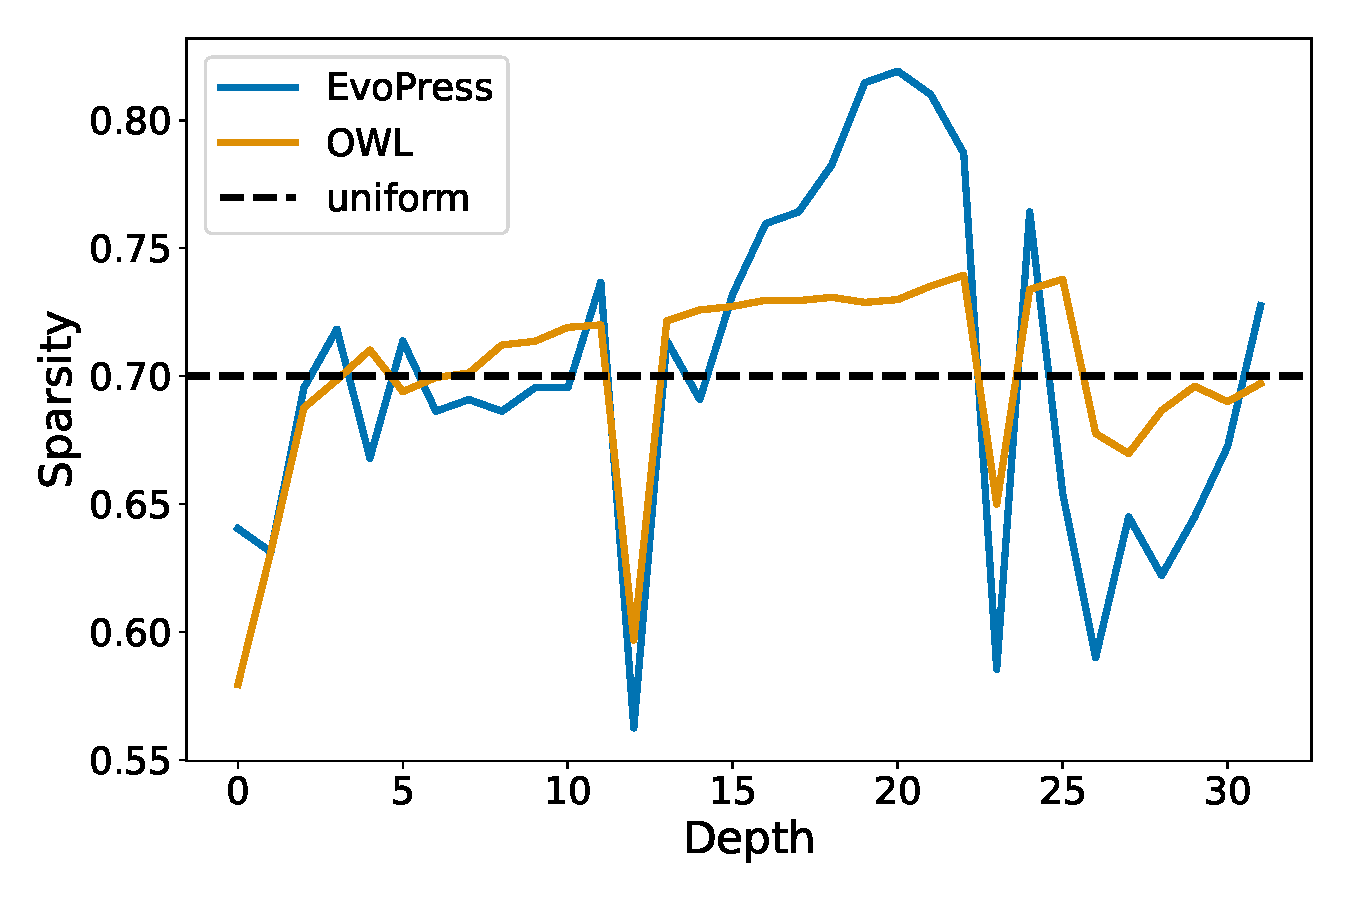
\includegraphics[width=\linewidth]{graphics/UnstructuredSparsity/sparsity-distribution-block-Meta-Llama-3.1-8B.pdf}
\captionof{figure}{Comparison of different block-level sparsity profiles for Llama-3.1-8B at 70\% sparsity.}
\label{fig:sparsity_distribution_block_Meta-Llama-3_1-8B}
\end{minipage}
\hfill
\begin{minipage}[htb]{0.48\linewidth}
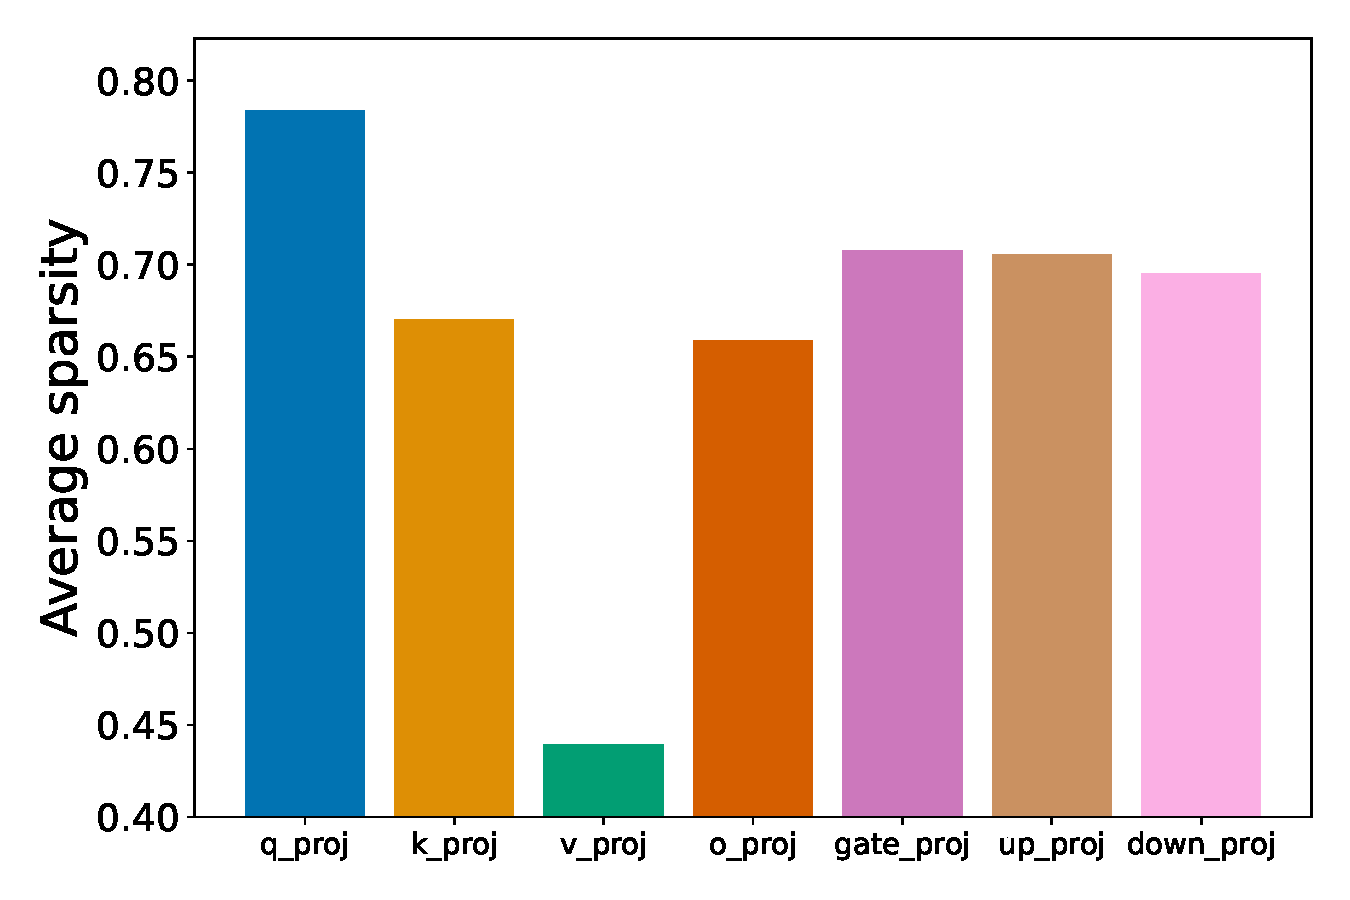
\includegraphics[width=\linewidth]{graphics/UnstructuredSparsity/sparsity-distribution-proj-Meta-Llama-3.1-8B.pdf}
\captionof{figure}{Average sparsity per projection type for Llama-3.1-8B at 70\% sparsity for \methodname{}.}
\label{fig:sparsity_distribution_proj_Meta-Llama-3_1-8B}
\end{minipage}


\section{Additional Quantization Results}
\subsection{2.25 Bit and 2.5 Bit}
\label{app:subsec:225and25}
In addition to the 3 bit results presented in Section~\ref{subsect:quantization}, we further evaluated \methodname{} under extreme quantization conditions, specifically testing it at 2.25 bit and 2.5 bit levels. As a baseline, we generated 32 random configurations combining 2 bit and 3 bit layers and selected the best performing setup. The results, as shown in Table~\ref{tab:extreme_quant}, demonstrate that \methodname{} significantly outperforms this baseline, highlighting its ability to achieve extreme quantization levels.

\begin{table}[htb]
\footnotesize
\centering
\setlength\tabcolsep{3pt}
\caption{Performance of EvoPress on 2.25 bit and 2.5 bit quantization.}\label{tab:quant_extreme}
\resizebox{0.75\textwidth}{!}{
\begin{tabular}{c|c|c|cc|ccccc|c}
    \toprule
    \bf{Model} & \bf{\# Bits} & \bf{Method} &\bf{Wiki2$\downarrow$} & \bf{C4$\downarrow$} & \bf{ArcC$\uparrow$} & \bf{ArcE$\uparrow$} & \bf{HS$\uparrow$} & \bf{PiQA$\uparrow$} & \bf{WG$\uparrow$} & \bf{Avg$\uparrow$} \\
    \midrule
     \multirow{5}{*}{Mistral-7B-v0.3}& \multirow{2}{*}{2.25} & Best of 32 & 11.53 & 18.32 & 30.1 & 59.6 & 44.5 & 69.4 & 56.8 & 52.1 \\
    &  & EvoPress   & \bf{8.63} & \bf{13.47} & 36.2 & 66.0 & 49.3 & 74.2 & 63.5 & \bf{57.8} \\
    \cmidrule{2-11}
    & \multirow{2}{*}{2.5} &  Best of 32 & 7.50 & 11.76 & 37.0 & 68.0 & 51.7 & 75.0 & 63.5 & 59.0 \\
     & &   EvoPress & \bf{6.60} & \bf{10.40} & 39.8 & 71.7 & 54.0 & 77.1 & 65.8 & \bf{61.7} \\
    \midrule 
     \multirow{5}{*}{Llama-2-7B}& \multirow{2}{*}{2.25} & Best of 32 & 13.18 & 18.19 & 24.8 & 50.2 & 40.3 & 66.8 & 56.1 & 47.7 \\
    &  & EvoPress   & \bf{9.82} & \bf{9.93} & 29.5 & 61.8 & 46.2 & 70.3 & 59.4 & \bf{53.4} \\
    \cmidrule{2-11}
    & \multirow{2}{*}{2.5} &  Best of 32 & 9.42 & 9.01 & 29.1 & 58.6 & 46.9 & 70.1 & 62.6 & 53.5 \\
     & &   EvoPress & \bf{8.03} & \bf{7.33} & 35.3 & 68.4 & 50.8 & 73.9 & 64.2 & \bf{58.5} \\
    \midrule 
    \multirow{5}{*}{Llama-3-8B}& \multirow{2}{*}{2.25} & Best of 32 & 149.85 & 432.96 & 21.2 & 29.1 & 28.1 & 55.6 & 49.8 & 36.8 \\
    &  & EvoPress   & \bf{23.93} & \bf{43.17} & 23.6 & 46.9 & 39.3 & 63.6 & 56.5 & \bf{46.0} \\
    \cmidrule{2-11}
    & \multirow{2}{*}{2.5} &  Best of 32 & 21.65 & 23.92 & 25.1 & 47.6 & 41.2 & 65.6 & 56.2 & 47.1 \\
     & &   EvoPress & \bf{13.93} & \bf{18.15} & 31.7 & 61.5 & 47.9 & 71.7 & 64.3 & \bf{55.4} \\
    \midrule
    \multirow{5}{*}{Llama-3.1-8B}& \multirow{2}{*}{2.25} & Best of 32 &  259.61 & 181.36 & 20.7 & 31.9 & 30.6 & 57.0 & 51.9 & 38.4 \\
    &  & EvoPress   & \bf{22.75} & \bf{33.58} & 26.7 & 48.9 & 40.2 & 63.4 & 55.7 & \bf{47.0} \\
    \cmidrule{2-11}
    & \multirow{2}{*}{2.5} &  Best of 32 & 35.33 & 37.09 & 24.1 & 48.4 & 41.7 & 62.7 & 54.5 & 46.3 \\
     & &   EvoPress & \bf{11.73} & \bf{19.03} & 32.2 & 63.3 & 47.5 & 71.8 & 62.3 & \bf{55.4} \\
    \midrule 
     \multirow{5}{*}{Phi-3-Medium}& \multirow{2}{*}{2.25} & Best of 32 & 14.20 & 18.19 & 28.9 & 46.8 & 40.0 & 61.8 & 53.1 & 46.1 \\
    &  & EvoPress   & \bf{10.48} & \bf{14.60} & 36.2 & 62.0 & 46.6 & 66.2 & 55.6 & \bf{53.3} \\
    \cmidrule{2-11}
    & \multirow{2}{*}{2.5} &  Best of 32 & 8.26 & 12.65 & 40.5 & 69.3 & 50.3 & 70.9 & 61.9 & 58.6 \\
     & &   EvoPress & \bf{7.12} & \bf{11.23} & 44.1 & 75.9 & 54.1 & 73.5 & 64.6 & \bf{62.4} \\
  \bottomrule
\end{tabular}
}
\label{tab:extreme_quant}
\end{table}


\subsection{Practical Convergence}
\label{subsec_app_quant_conv}
Similar to unstructured sparsity, \methodname{} also demonstrates rapid convergence when applied to quantization. As shown in Figure~\ref{fig:conv_quant}, the majority of improvements occur within two GPU hours, with full convergence achieved after approximately eight GPU hours. If needed, this optimization time could be further shortened by tuning the hyperparameters, similarly to the ``super-fast'' version for unstructured sparsity discussed in Section~\ref{subsect:sparsity}. However, we observed that the convergence dynamics are less smooth compared to unstructured sparsity, likely due to the limited number of quantization levels available (practically only 2, 3, and 4 bit are used), which results in a less smooth fitness landscape.

\begin{figure}[htb]
    \centering
    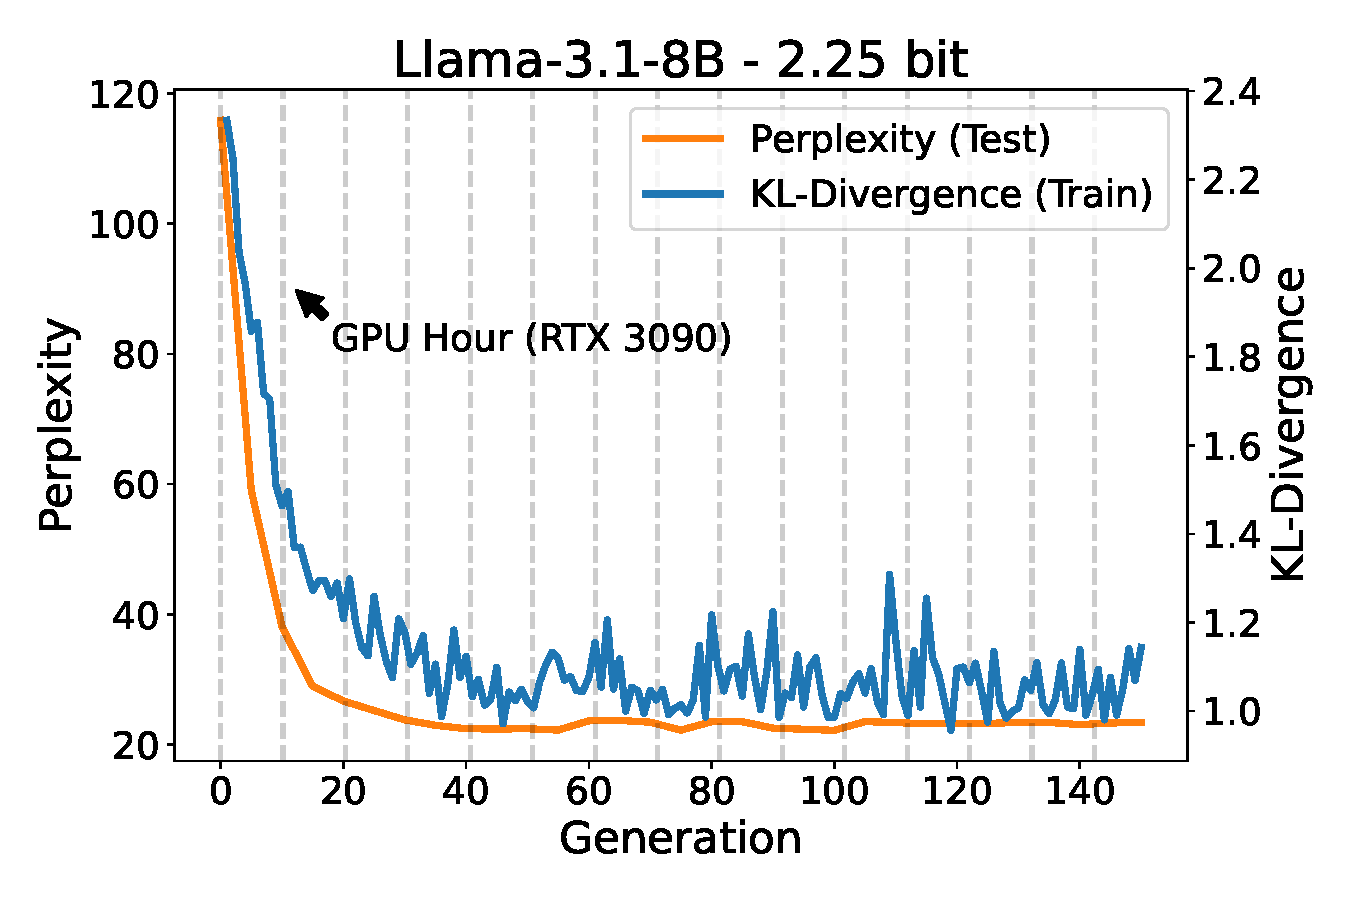
\includegraphics[width=0.48\linewidth]{graphics/Convergence/Convergence_Llama-3.1-8B_2.25bit.pdf}
    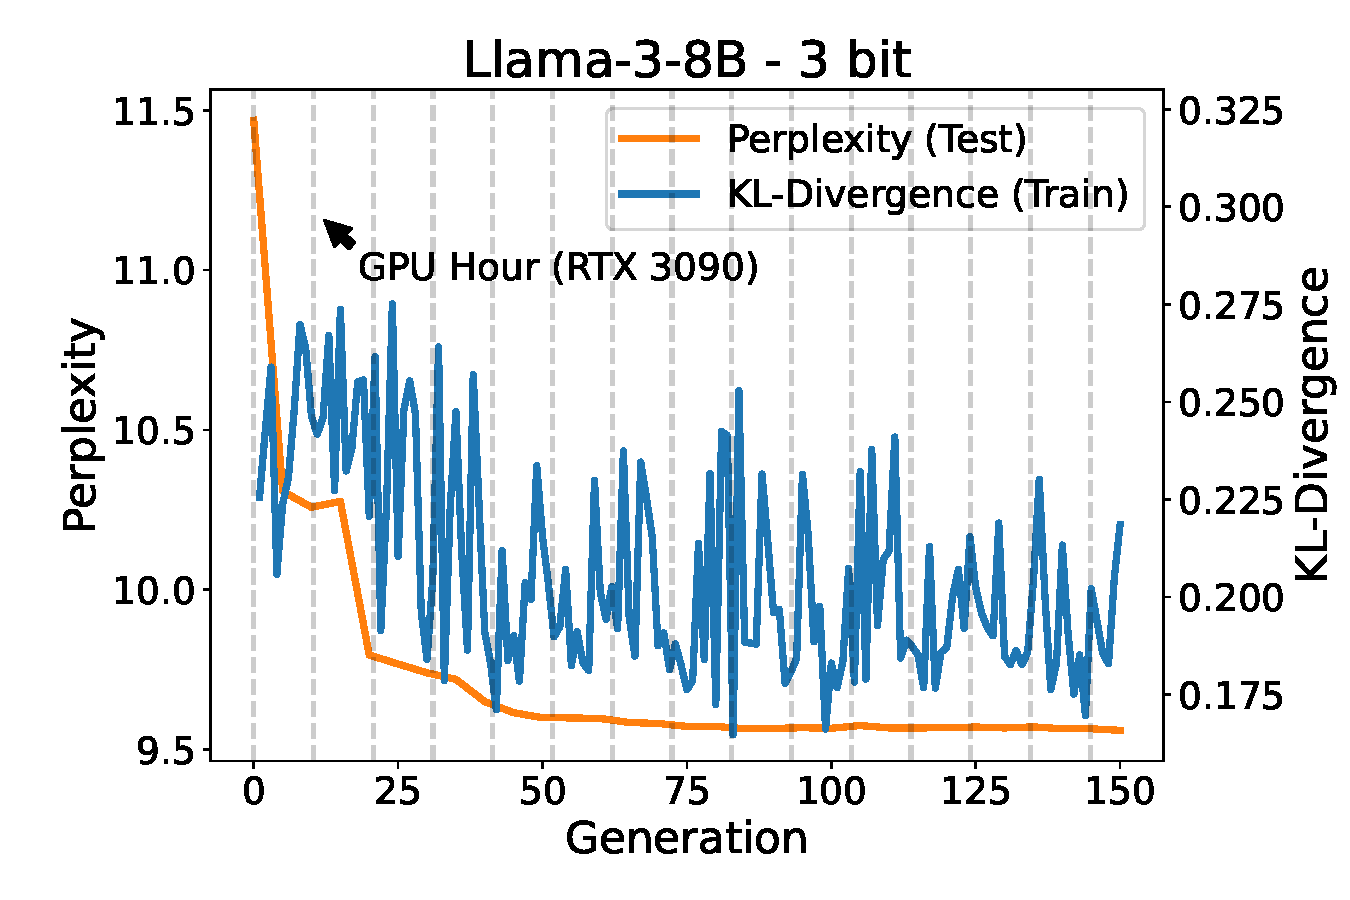
\includegraphics[width=0.48\linewidth]{graphics/Convergence/Convergence_Llama-3-8B_3bit.pdf}
    \caption{Convergence of \methodname{} for 2.25 bit quantization on Llama-3.1-8B (left) and 3 bit quantization on Llama-3-8B (right).} 
    \label{fig:conv_quant}
\end{figure}

\subsection{Quantization Profiles}

In this section, we visualize a quantization profile determined by \methodname{}. As shown, \methodname{} maintains a relatively uniform quantization bitwidth allocation across the model. Interestingly, while the second and the two last blocks are less compressed, the first block undergoes significantly higher compression. This suggests that ``saliency'' does not directly equate to block importance but rather depends on the specific compression method used. Additionally, similar to the profiles for unstructured sparsity, we observe a transfer of capacity to \texttt{v\_proj}.

\begin{minipage}[htb]{0.45\linewidth}
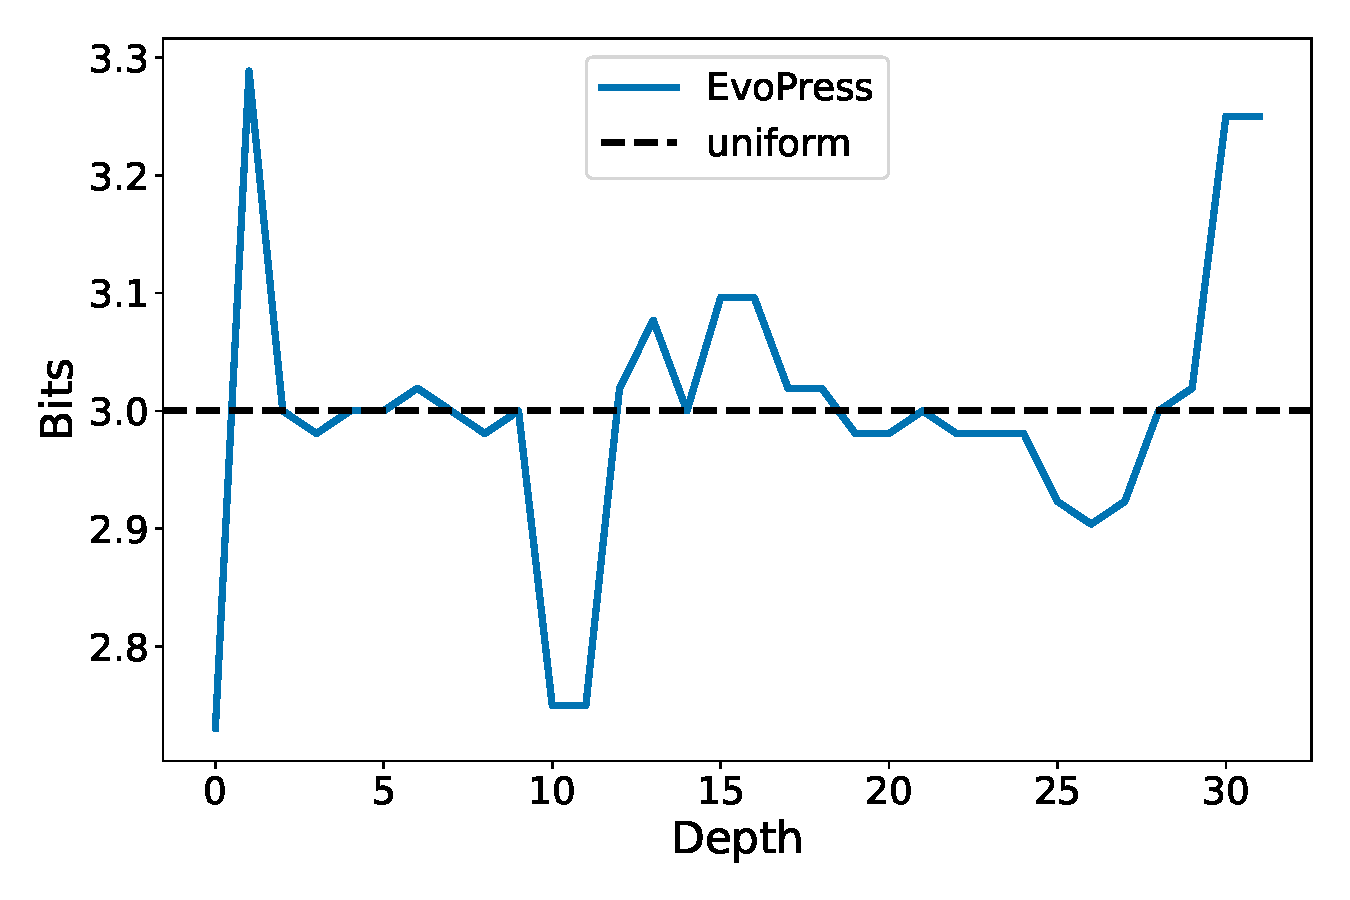
\includegraphics[width=\linewidth]{graphics/Quantization/quantization-distribution-block-Meta-Llama-3.1-8B-3bit.pdf}
\captionof{figure}{Block-level quantization profiles for Llama-3.1-8B at 3 bit compression on average.}
\label{fig:quantization_distribution_block_Meta-Llama-3_1-8B}
\end{minipage}
\hfill
\begin{minipage}[htb]{0.45\linewidth}
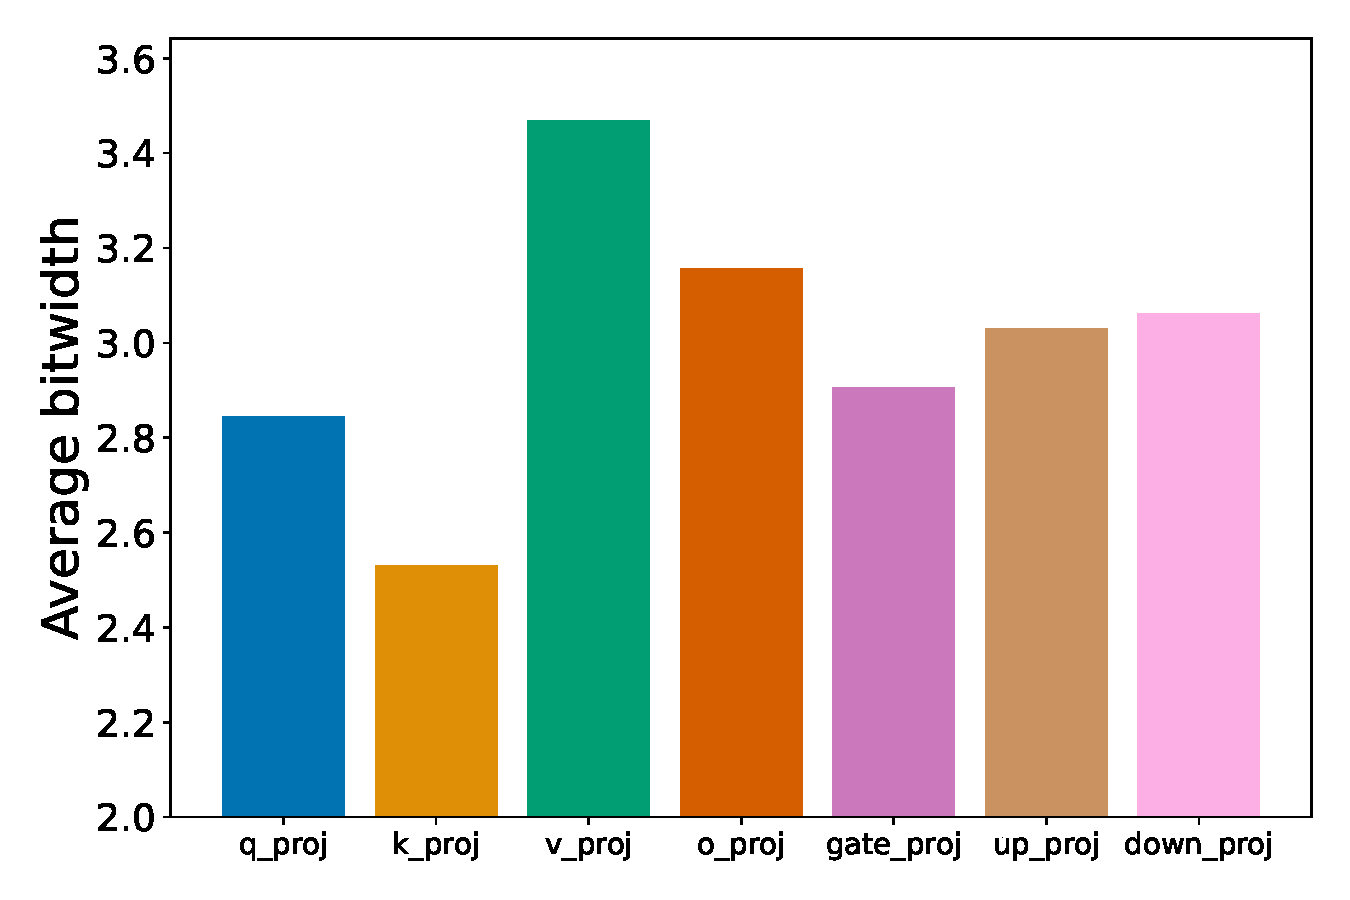
\includegraphics[width=\linewidth]{graphics/Quantization/quantization-distribution-proj-Meta-Llama-3.1-8B-3bit.pdf}

\captionof{figure}{Average bitwidth per projection type for Llama-3.1-8B at 3 bit compression on average.}
\label{fig:quantization_distribution_proj_Meta-Llama-3_1-8B}
\end{minipage}

\section{Running Time Comparisons}
\label{app:sec:running_time_comp}
In our main results, we did not include a stopping criteria into the optimization process, but instead continued the search well beyond convergence to observe the convergence behavior. Here, we include a simple stopping criteria to our search, which terminates the search whenever the perplexity on the training set has not improved in the last 20 generations. Based on this version we compare the runtime requirements of \methodname{} with baseline methods. However, it should be noted that the amount of data used impacts both runtime and compression quality (with specific trade-offs being method-dependent), meaning one can generally trade-off both objectives, which makes runtime comparison difficult. 

In Table~\ref{tab:dropping_comparison} we compare \methodname{} for block dropping to various baseline methods on Llama-2-7B, where we, additionally to the main results, also compare against the iterative search methods BlockPruner \cite{zhong2024blockpruner} and SLEB \cite{song2024sleb}. As the results show, \methodname{} achieves the best compressed models across all sparsity ratios, while being quicker than other search methods. Scoring-based methods are considerably faster than the search-based methods, but produce significantly worse models.



\begin{table}[ht]
\centering
\footnotesize
\caption{Comparison of various depth pruning methods at different sparsities. We report
the runtime on a single NVIDIA RTX 4090 GPU. Note that some methods perform forward passes on a strongly depth-pruned model, which explains the runtime difference for EvoPress on 50\% and 12.5\% sparsity.}
\label{tab:dropping_comparison}
\begin{tabular}{cc|ccc|cc}
\toprule
\textbf{Sparsity} & \textbf{Method} & \textbf{Fineweb$\downarrow$} & \textbf{Wiki2$\downarrow$} & \textbf{C4$\downarrow$} & \textbf{Runtime} & \textbf{Fwd. Passes (Tokens)} \\
\midrule
0\%   & -                                & 6.40  & 5.12  & 6.99  & -      & -      \\
\midrule
12.5\% & ShortGPT                         & 9.30  & 8.86  & 10.78 & 46s    & 65K    \\
12.5\% & Cosine Similarity (Window)          & 8.51  & 7.53  & 9.82  & 46s    & 65K    \\
12.5\% & Weight Subcloning               & 9.60  & 9.09  & 11.06 & 49s    & 65K    \\
12.5\% & ShortenedLlama                  & 8.57  & 7.68  & 10.44 & 8min   & 2.1M   \\
12.5\% & SLEB                             & 7.71  & 6.51  & 8.78  & 70min  & 18.8M  \\
11.4\% & BlockPruner                     & 7.88  & 7.88  & 8.86  & 100min & 26.6M  \\
12.5\% & EvoPress                         & \bf{7.61}  & \bf{6.41}  & \bf{8.67}  & 58min  & 12.4M  \\
\midrule
25\%   & ShortGPT                         & 21.16 & 23.41 & 30.30 & 44s    & 65K    \\
25\%   & Cosine Similarity (Window)          & 17.37 & 16.60 & 21.04 & 46s    & 65K    \\
25\%   & Weight Subcloning               & 21.16 & 23.41 & 30.30 & 49s    & 65K    \\
25\%   & ShortenedLlama                  & 11.81 & 13.86 & 14.08 & 8min   & 2.1M   \\
25\%   & SLEB                             & 10.21 & \bf{9.45}  & 12.03 & 122min & 35.2M  \\
25\%   & BlockPruner                     & 11.31 & 12.49 & 13.32 & 152min & 42.8M  \\
25\%   & EvoPress                         & \bf{10.06} & 10.31 & \bf{11.99} & 44min  & 10.0M  \\
\midrule
37.5\% & ShortGPT                         & 54.07 & 70.94 & 63.51 & 44s    & 65K    \\
37.5\% & Cosine Similarity (Window)         & 151.10 & 192.07 & 212.60 & 45s   & 65K    \\
37.5\% & Weight Subcloning               & 54.07 & 70.94 & 63.51 & 49s    & 65K    \\
37.5\% & ShortenedLlama                  & 20.37 & 35.37 & 26.07 & 8min   & 2.1M   \\
37.5\% & SLEB                             & 17.29 & 19.57 & 20.91 & 159min & 49.1M  \\
36.4\% & BlockPruner                     & 19.41 & 28.75 & 22.44 & 185min & 54.8M  \\
37.5\% & EvoPress                         & \bf{16.09} & \bf{17.44} & \bf{19.87} & 53min  & 19.7M  \\
\midrule
50\%   & ShortGPT                         & 180.51 & 226.14 & 171.04 & 44s    & 65K    \\
50\%   & Cosine Similarity (Window)         & 3611.06 & 4570.15 & 2876.83 & 45s   & 65K    \\
50\%   & Weight Subcloning               & 180.51 & 226.14 & 141.04 & 49s    & 65K    \\
50\%   & ShortenedLlama                  & 68.79  & 145.78 & 87.40  & 8min   & 2.1M   \\
50\%   & SLEB                             & 51.30  & 117.21 & 58.56  & 184min & 60.1M  \\
48.9\% & BlockPruner                     & 52.28  & 97.23  & 60.47  & 208min & 64.9M  \\
50\%   & EvoPress                         & \bf{34.20}  & \bf{47.15}  & \bf{40.10}  & 31min  & 12.4M  \\
\bottomrule
\end{tabular}
\end{table}


In Table~\ref{besa_comparison} we provide a comparison of EvoPress with BESA \cite{xu2024besapruninglargelanguage}, a method for non-uniform sparsity allocation. BESA performs gradient-descent based search for rowwise sparsity allocation using straight-through-estimation \cite{bengio2013estimating}, with uniform sparsity on a per-block level. Therefore, both methods are not fully comparable, as \methodname{} searches for layerwise sparsities globally (across the entire model, not just blockwise), while keeping per-row sparsities uniform. We demonstrate that both methods are complementary by performing a two-stage search, first, for blockwise sparsities using EvoPress, then, for rowwise sparsities with fixed per-block sparsity using BESA. This merged version produces best results on 50\% and 60\% sparsity, while it performs slightly worse than pure \methodname{} on 70\% sparsity. For a fair comparison, we search on top of a Wanda \cite{wanda} layer database for all methods. The runtime requirements for both BESA and \methodname{} are similar, as there is an additional hyperparameter sweep for BESA, which is not provided in the author's implementation (authors provide tuned coefficients). Similarly, we have not included OWL in this comparison, as the authors have not provided instructions on how  hyperparameters were obtained.


\begin{table}[h!]
\centering
\begin{threeparttable}

\caption{Comparison of EvoPress with uniform pruning and BESA on Llama-2-7B. Both EvoPress as well as BESA (layerwise) operate on a layer database generated via Wanda. BESA (rowwise) additionally learns per-output-channel sparsities, which target a different dimension of the compression space than EvoPress's layerwise allocation. EvoPress+BESA applies BESA using the average per-block sparsities found from running EvoPress, showing that both methods can work complementary. Here, we use the lightweight version of EvoPress with early stopping.}
\label{besa_comparison}
\begin{tabular}{ccc|ccc|c}
\toprule
\textbf{Sparsity} & \textbf{Method} & \textbf{Non-Uniformity} & \textbf{Fineweb$\downarrow$} & \textbf{Wiki2$\downarrow$} & \textbf{C4$\downarrow$} & \textbf{Runtime} \\
\midrule
50.00 & Uniform & N/A & 7.60 & 6.41 & 8.97 & - \\
\textcolor{red}{49.79} & BESA & Layerwise & 7.55 & 6.32 & 8.93 & 16min* \\
50.00 & EvoPress & Layerwise & 7.48 & 6.28 & 8.79 & 87min \\
\textcolor{red}{49.70} & BESA & Rowwise & 7.39 & 6.19 & 8.72 & 33min* \\
\textcolor{red}{49.72} & EvoPress+BESA & Rowwise & \textbf{7.37} & \textbf{6.16} & \textbf{8.71} & 120min \\
\midrule
60.00 & Uniform & N/A & 10.22 & 9.56 & 12.95 & - \\
\textcolor{red}{59.46} & BESA & Layerwise & 9.82 & 8.80 & 12.38 & 16min* \\
\textcolor{red}{58.91} & EvoPress & Layerwise & 8.75 & 8.03 & 11.94 & 102min \\
59.99 & EvoPress & Layerwise & 9.01 & 8.66 & 10.96 & 94min \\
\textcolor{red}{58.90} & BESA & Rowwise & 9.15 & 8.11 & 11.88 & 33min* \\
\textcolor{red}{59.12} & EvoPress+BESA & Rowwise & \textbf{8.59} & \textbf{7.58} & \textbf{10.58} & 135min* \\
\midrule
70.00 & Uniform & N/A & 64.02 & 136.53 & 97.53 & - \\
69.97 & BESA & Layerwise & 52.65 & 66.51 & 67.58 & 16min* \\
\textcolor{red}{68.52} & EvoPress & Layerwise & \textbf{13.53} & 15.61 & \textbf{16.90} & 111min \\
69.99 & EvoPress & Layerwise & 15.55 & 24.04 & 19.54 & 120min \\
\textcolor{red}{68.51} & BESA & Rowwise & 16.53 & 17.79 & 24.09 & 33min* \\
\textcolor{red}{68.03} & EvoPress+BESA & Rowwise & 13.83 & \textbf{14.19} & 19.52 & 144min* \\
\bottomrule
\end{tabular}
\begin{tablenotes}
\footnotesize
\item[\textcolor{red}{\textbullet}] Sparsity values in \textcolor{red}{red} are more than 0.5\% below the target. They are a result of BESA only enforcing a soft constraint on the effective sparsity.
\item[*] BESA runtimes do not include the hyperparameter sweep over `-d-coef`.
\end{tablenotes}
\end{threeparttable}
\end{table}



% \section{Schematic Visualization}

% We provide a schematic illustration of EvoPress in Figure~\ref{fig:evopress_illustration}.

% \begin{figure}[htb]
% \centering

%     \includegraphics[width=0.7\linewidth]{graphics/Schematic/EvoPress-visualization.pdf}

%   \caption{Schematic illustration of EvoPress search. Intially, a set of candidates is sampled. Then, a fraction of the fittest among them is selected at each elimination round. In the last selection round, the parent is added to the population for elitism. Finally, the last remaining search point is made the new parent.}
%     \label{fig:evopress_illustration}
% \end{figure}

